% ============================================================
%  Dispensa 03c: PCA sulle Curve EIOPA (Risk-Free Rate)
%               Variante della dispensa 03 su fonte dati diversa
%               (curva regolamentare EIOPA anziché ECB)
%  Corso di Calcolo Numerico — Laboratorio
%  Università degli Studi di Verona — A.A. 2026–2027
% ============================================================
\documentclass[11pt,a4paper]{article}

\usepackage[T1]{fontenc}
\usepackage[utf8]{inputenc}
\usepackage[italian]{babel}
\usepackage{lmodern}
\usepackage{amsmath,amssymb,amsthm,mathtools}
\usepackage{geometry}
\usepackage{booktabs}
\usepackage{array}
\usepackage{enumitem}
\usepackage{graphicx}
\usepackage{xcolor}
\usepackage{hyperref}
\usepackage{float}
\usepackage{fancyvrb}
\usepackage{tcolorbox}
\tcbuselibrary{breakable}
\usepackage{titlesec}

% le figure sono prodotte da R/03c_pca_eiopa.R in output/03c_pca_eiopa/
\graphicspath{{}}

\geometry{top=2.5cm,bottom=2.5cm,left=2.8cm,right=2.8cm}
\setlist[itemize]{topsep=4pt,itemsep=2pt,parsep=0pt}
\setlist[enumerate]{topsep=4pt,itemsep=2pt,parsep=0pt}
\hypersetup{colorlinks=true,linkcolor=blue!55!black,urlcolor=blue!55!black}

\titleformat{\section}{\large\bfseries}{\thesection.}{0.55em}{}[{\vspace{1pt}\titlerule[0.4pt]}]
\titleformat{\subsection}{\normalsize\bfseries}{\thesubsection.}{0.55em}{}
\titleformat{\subsubsection}{\small\bfseries\itshape}{\thesubsubsection.}{0.5em}{}

%--- macro acronimi
\newcommand{\UFR}{\ensuremath{\mathrm{UFR}}}
\newcommand{\LLP}{\ensuremath{\mathrm{LLP}}}
\newcommand{\CRA}{\ensuremath{\mathrm{CRA}}}

%--- ambienti teorema
\theoremstyle{plain}
\newtheorem{teorema}{Teorema}[section]
\newtheorem{proposizione}[teorema]{Proposizione}
\theoremstyle{definition}
\newtheorem{definizione}[teorema]{Definizione}
\newtheorem{esempio}[teorema]{Esempio}
\theoremstyle{remark}
\newtheorem*{osservazione}{Osservazione}
\newtheorem*{attenzione}{Nota numerica}

%--- box colorati
\tcbset{
  mybase/.style={
    colback=gray!5, colframe=gray!40,
    boxrule=0.4pt, arc=2pt,
    left=7pt, right=7pt, top=5pt, bottom=5pt,
    fonttitle=\small\bfseries
  }
}
\newtcolorbox{keybox}[1][Concetto chiave]{mybase,
  colframe=blue!40!black, colback=blue!4, title={#1}}
\newtcolorbox{algobox}[1][Algoritmo]{mybase,
  colframe=teal!50!black, colback=teal!4, title={#1}}
\newtcolorbox{warningbox}{mybase,
  colframe=orange!70!black, colback=orange!5}
\newtcolorbox{codebox}[1][Codice R]{mybase,
  colframe=green!40!black, colback=green!3, title={#1}}

% ============================================================
\title{%
  \textbf{PCA sulla Curva Risk-Free EIOPA (Solvency II)}\\[6pt]
  \large Teoria, Implementazione in R e Interpretazione Economica\\[4pt]
}
\author{Laboratorio di Calcolo Numerico --- Laurea Triennale in Matematica Applicata\\
  Universit\`a degli Studi di Verona\\[2pt]
  Anno Accademico 2026--2027}
\date{}

\begin{document}
\maketitle
\tableofcontents
\newpage

% ============================================================
\section{Introduzione e obiettivi}
% ============================================================

\subsection{Il problema}

La \textbf{curva dei tassi di interesse} (o struttura a termine) associa a ogni
scadenza $T$ un tasso di rendimento $r(T)$ per titoli privi di rischio. La curva
cambia ogni giorno in risposta a decisioni di politica monetaria, aspettative di
inflazione e fattori macroeconomici.

In questa dispensa analizziamo la \textbf{curva risk-free EUR pubblicata
mensilmente da EIOPA} ai fini della direttiva Solvency~II, considerando le
scadenze da 1 a 20 anni, cio\`e fino all'\emph{ultimo punto liquido} ($\LLP$)
della valuta euro. L'obiettivo \`e comprendere e sintetizzare i principali
movimenti osservati nella curva nel corso del tempo.

Monitorare direttamente tutte le scadenze della curva richiederebbe di gestire
almeno 20 variabili (una per ogni maturity). Nel caso EIOPA il problema
dimensionale non \`e ipotetico ma \`e il caso ordinario: la curva ufficiale
\`e pubblicata su \textbf{150 scadenze}. Qui ci limitiamo alle prime 20
(Sezione~\ref{sec:origine-dati}), ma il metodo si applica identico a tutte.

Per questo motivo, \`e utile cercare una rappresentazione pi\`u compatta, ovvero
individuare i \emph{movimenti fondamentali} della curva che, combinati tra loro,
spiegano la maggior parte delle variazioni osservate.

In questa dispensa presentiamo la \textbf{Principal Component Analysis (PCA)},
implementata tramite la \textbf{Singular Value Decomposition (SVD)}, che permette
di identificare e quantificare le principali variazioni della curva dei tassi.
Vedremo come, grazie a questa tecnica, sia possibile descrivere l'evoluzione
della curva nel tempo utilizzando solo poche componenti principali, facilitando
l'analisi e l'interpretazione dei dati.

Nella dispensa \`e inoltre riportato il codice utilizzato per l'elaborazione dei
dati, scritto nel linguaggio R.

\medskip
Le dispense~01 e~03 hanno mostrato \textbf{come si costruisce} la curva EIOPA
(bootstrap ed estrapolazione la prima, Smith--Wilson la seconda), a partire dai
tassi swap di un singolo mese. Questa dispensa cambia punto di vista: prendiamo
per date le curve gi\`a pubblicate e ci chiediamo \textbf{come si muovono nel
tempo}.

\subsection{La frequenza mensile: un vincolo del dato, non una scelta}
\label{sec:motivazione-mensile}

A differenza della BCE, che pubblica la curva ogni giorno lavorativo,
\textbf{EIOPA pubblica una sola curva al mese}, riferita all'ultimo giorno di
calendario del mese. La frequenza mensile non \`e quindi una scelta
dell'analista ma una caratteristica del dato regolamentare: non esiste alcun
passo di aggregazione da giornaliero a mensile, e non esiste la scelta
arbitraria --- presente invece nell'analisi BCE della dispensa~03 --- tra
ultima osservazione del mese e media mensile. La data \`e fissata dal
regolatore ed \`e la stessa su cui \emph{tutte} le imprese assicurative europee
valutano le riserve tecniche di quel mese.

Dal punto di vista dell'analisi economica questa frequenza \`e anche quella
giusta: l'obiettivo non \`e catturare movimenti di brevissimo periodo o
dinamiche di microstruttura, bens\`i descrivere l'evoluzione della curva dei
rendimenti su orizzonti temporali pi\`u ampi, rilevanti per analisi prospettiche
e di scenario. L'utilizzo di variazioni giornaliere risulta pi\`u adatto ad
applicazioni di trading o gestione operativa ad alta frequenza, mentre offre un
contenuto informativo limitato per un'analisi strutturale dei fattori della curva.

Le osservazioni mensili permettono di cogliere chiaramente i principali eventi
macro-finanziari del campione: il referendum sulla Brexit (giugno 2016), lo
shock pandemico e il varo del PEPP (marzo 2020), la svolta restrittiva della BCE
e l'uscita dai tassi negativi (febbraio 2022), il picco dei tassi ufficiali
(settembre 2023) e l'avvio del ciclo di tagli (giugno 2024).

Il prezzo di questa scelta \`e la lunghezza del campione: \textbf{127 curve
mensili} (dicembre 2015 -- giugno 2026, senza interruzioni) contro le oltre 250
osservazioni mensili disponibili per la curva BCE.

\subsection{Origine dei dati}
\label{sec:origine-dati}

I dati provengono dal \textbf{Risk-Free Rate register} di EIOPA%
\footnote{\url{https://www.eiopa.europa.eu/tools-and-data/risk-free-interest-rate-term-structures}.
Gli archivi mensili usati in questa dispensa sono in \texttt{dati/eiopa\_zips/}.}
(\emph{European Insurance and Occupational Pensions Authority}), l'autorit\`a
europea di vigilanza sulle assicurazioni.

Ogni mese EIOPA pubblica la struttura a termine dei tassi risk-free che
\textbf{tutte} le imprese di assicurazione europee devono utilizzare per
scontare le riserve tecniche ai fini di Solvency~II. La curva non \`e quindi una
stima statistica come quella della BCE, ma un \textbf{dato regolamentare}: \`e
unica, obbligatoria e identica per tutti gli operatori.

\paragraph{Sottostante: swap, non titoli di Stato.}
La differenza pi\`u importante rispetto alla curva BCE della dispensa~03 \`e il
mercato di riferimento. La BCE stima la curva sui rendimenti dei
\emph{titoli di Stato} dell'area euro con rating AAA; EIOPA parte invece dai
\textbf{tassi swap di tasso di interesse} (par swap rate) denominati in euro.

\paragraph{Credit Risk Adjustment.}
Poich\'e i tassi swap incorporano un residuo rischio di controparte bancaria, al
tasso di mercato viene sottratto il \textbf{Credit Risk Adjustment} ($\CRA$),
pari a 10 punti base per l'euro e costante su tutto il campione.

\paragraph{Scadenze quotate e Last Liquid Point.}
Il mercato quota gli swap EUR soltanto su un insieme di scadenze
\emph{Deep, Liquid and Transparent} (DLT). Per l'euro si tratta di
\textbf{15 nodi} (cfr.\ dispensa~03):
\[
  \{1,2,3,4,5,6,7,8,9,10,11,12,13,\,15,\,20\}\ \text{anni},
\]
mentre le scadenze 14, 16, 17, 18 e 19 anni sono \textbf{interpolate} dal
metodo Smith--Wilson, che riproduce esattamente i prezzi degli strumenti
quotati e riempie il resto con il criterio di minima energia.

Oltre il \textbf{Last Liquid Point} ($\LLP = 20$ anni per l'euro) la curva non
\`e pi\`u interpolata ma \textbf{estrapolata} verso l'\emph{Ultimate Forward
Rate} ($\UFR$).

\begin{keybox}[La finestra 1--20 anni]
La finestra $1$--$20$ anni che analizziamo coincide esattamente con la parte
\textbf{liquida} della curva: l'estrapolazione verso l'$\UFR$, oggetto delle
dispense~01 e~03, riguarda le scadenze oltre il ventesimo anno e
\textbf{non entra} in questa analisi.
\end{keybox}

\paragraph{Parametri della curva sul campione.}
I metadati pubblicati insieme a ogni curva sono riassunti in
Tabella~\ref{tab:parametri}.

\begin{table}[H]
\centering
\small
\renewcommand{\arraystretch}{1.25}
\begin{tabular}{lp{9.2cm}}
\toprule
Parametro & Valore sul campione (dic.\ 2015 -- giu.\ 2026) \\
\midrule
$\LLP$ & 20 anni (costante) \\
$\CRA$ & 10 punti base (costante) \\
Convergence point & 40 anni (costante) \\
$\UFR$ & $4{,}20\%$ fino a dic.\ 2017; poi $4{,}05\%$ (gen.\ 2018),
         $3{,}90\%$ (2019), $3{,}75\%$ (2020), $3{,}60\%$ (2021),
         $3{,}45\%$ (2022), $3{,}30\%$ (da gen.\ 2024) \\
$\alpha$ & ricalibrato ogni mese; intervallo osservato $0{,}050$--$0{,}138$ \\
\bottomrule
\end{tabular}
\caption{Parametri regolamentari della curva EUR sul campione analizzato,
estratti dai metadati di ciascun archivio mensile.}
\label{tab:parametri}
\end{table}

\paragraph{Curva ``no VA''.}
Utilizziamo la curva \textbf{senza \emph{volatility adjustment}} (foglio
\texttt{RFR\_spot\_no\_VA}): il VA \`e una maggiorazione che dipende dal
portafoglio della singola impresa, mentre la curva senza VA \`e la curva
risk-free di base, metodologicamente pulita.

\begin{warningbox}
\textbf{Convenzione di capitalizzazione.}
La BCE pubblica tassi in \textbf{capitalizzazione continua},
$P(0,T)=e^{-r(T)T}$ (dispensa~03). EIOPA pubblica tassi in
\textbf{capitalizzazione annua composta}, $P(0,T)=(1+r(T))^{-T}$,
coerentemente con le dispense~01 e~03. Le due convenzioni differiscono di
$O(r^2/2)$: circa 5~pb a un livello del $3\%$. Per l'analisi delle
\emph{variazioni} la differenza si riduce a un riscalamento di fattore
$\approx(1+r)^{-1}$, irrilevante per la struttura fattoriale; ma le curve
delle due dispense \textbf{non sono direttamente sovrapponibili} senza
conversione.
\end{warningbox}

\noindent Per le definizioni di fattore di sconto, tasso spot e tasso forward si
rimanda alla dispensa~03.

\subsection{Dataset}

I dati grezzi sono i \textbf{127 archivi} \texttt{.zip} contenuti in
\texttt{dati/eiopa\_zips/}, uno per ogni mese da dicembre 2015 a giugno 2026.
Ciascun archivio contiene il file
\texttt{EIOPA\_RFR\_\textit{AAAAMMGG}\_Term\_Structures.xlsx}, il cui foglio
\texttt{RFR\_spot\_no\_VA} riporta le curve di tutti i paesi: la colonna
\texttt{Euro} contiene i tassi che ci interessano, sulle scadenze da 1 a 150
anni.

Lo script \texttt{R/03c\_pca\_eiopa\_prep.R} estrae le prime 20 scadenze da tutti
gli archivi e produce il file \texttt{dati/03c\_eiopa\_spot.xlsx}
(fogli \texttt{PCA\_Input} e \texttt{Metadata}), che \`e l'input dell'analisi
(dettagli e codice R nella Sezione~\ref{sec:estrazione}).

\begin{warningbox}
\textbf{Unit\`a di misura.}
Gli archivi EIOPA esprimono i tassi in forma \textbf{decimale}
($0{,}02592$ significa $2{,}592\%$), mentre il file BCE della dispensa~03 li
esprime in \textbf{punti percentuali} ($2{,}592$). In questa dispensa adottiamo
la convenzione \textbf{percentuale} su tutta la pipeline: la conversione avviene
una volta sola, in \texttt{03c\_pca\_eiopa\_prep.R}. Un punto base vale quindi
$0{,}01$ nelle unit\`a di lavoro, e tutti i grafici in pb si ottengono
moltiplicando per~$100$.
\end{warningbox}

% ============================================================
\section{Prerequisiti matematici: SVD e approssimazione ottimale}
% ============================================================

In questa sezione presentiamo gli strumenti matematici necessari per la PCA,
organizzati attorno a una domanda centrale:

\begin{keybox}[Il problema fondamentale]
Data una matrice $X \in \mathbb{R}^{m \times n}$ (ad esempio le variazioni
mensili della curva dei tassi), come possiamo rappresentarla in modo
\emph{compatto} usando solo $k \ll n$ ``direzioni'' fondamentali, perdendo
la minima quantità possibile di informazione?
\end{keybox}

La risposta a questa domanda passa attraverso tre risultati:
\begin{enumerate}
  \item la \textbf{SVD} fattorizza qualsiasi matrice in componenti ordinate
        per importanza;
  \item il teorema di \textbf{Eckart--Young--Mirsky} garantisce che troncare
        la SVD alle prime $k$ componenti dà la migliore approssimazione
        possibile di rango $k$;
  \item la \textbf{norma di Frobenius} usata in questo teorema coincide
        (a meno di costanti) con la \emph{varianza totale}, quindi
        ``miglior approssimazione'' significa ``massima varianza spiegata''.
\end{enumerate}

\medskip

% ------------------------------------------------------------
\subsection{Decomposizione ai Valori Singolari (SVD)}
% ------------------------------------------------------------

\begin{teorema}[Esistenza e unicità della SVD]
\label{thm:svd}
Per ogni matrice $A \in \mathbb{R}^{m \times n}$ esistono:
\begin{itemize}
  \item una matrice ortogonale $U \in \mathbb{R}^{m \times m}$ (colonne = \textbf{vettori singolari sinistri});
  \item una matrice ortogonale $V \in \mathbb{R}^{n \times n}$ (colonne = \textbf{vettori singolari destri});
  \item una matrice diagonale $\Sigma \in \mathbb{R}^{m \times n}$ con elementi
        $\sigma_1 \geq \sigma_2 \geq \cdots \geq \sigma_{\min(m,n)} \geq 0$
        (\textbf{valori singolari});
\end{itemize}
tali che $A = U \Sigma V^T$. I valori singolari sono unici; i vettori singolari
sono unici a meno di segno quando i $\sigma_i$ sono distinti.
\end{teorema}

\paragraph{Interpretazione geometrica.}
La SVD scompone l'azione di $A$ in tre passi:
\[
  \mathbf{x} \;\xrightarrow{V^T}\; \text{rotazione}
  \;\xrightarrow{\Sigma}\; \text{scaling per asse}
  \;\xrightarrow{U}\; \text{rotazione}.
\]
I valori singolari $\sigma_i$ misurano quanto $A$ ``allunga'' lungo ciascun asse
principale: $\sigma_1$ è la direzione di massimo allungamento, $\sigma_n$ quella
di minimo. Nel contesto PCA:
\begin{itemize}
  \item le colonne di $V$ sono le \textbf{direzioni principali} (loadings);
  \item le colonne di $U$, scalate per $\sigma_i$, danno gli \textbf{scores};
  \item $\sigma_i^2$ è proporzionale alla \textbf{varianza} lungo la $i$-esima direzione.
\end{itemize}

% ------------------------------------------------------------
\subsection{La norma di Frobenius}
% ------------------------------------------------------------

Definiamo la \textbf{norma di Frobenius} come segue:
\[
  \|A\|_F = \sqrt{\sum_{i,j} a_{ij}^2} = \sqrt{\operatorname{tr}(A^T A)}.
\]

\begin{proposizione}[Frobenius e valori singolari]
\label{prop:frob}
Per ogni matrice $A$ con valori singolari $\sigma_1, \ldots, \sigma_r$ (dove
$r = \operatorname{rk}(A)$):
\begin{equation}
  \|A\|_F^2 = \sigma_1^2 + \sigma_2^2 + \cdots + \sigma_r^2.
  \label{eq:frob_svd}
\end{equation}
\end{proposizione}

% ------------------------------------------------------------
\subsection{Il teorema di Eckart--Young--Mirsky: ottimalità della SVD troncata}
% ------------------------------------------------------------

\begin{teorema}[Eckart--Young--Mirsky, 1936]
\label{thm:ey}
Sia $A = U \Sigma V^T$ la SVD di $A$, e sia
\[
  A_k = \sum_{i=1}^{k} \sigma_i \, \mathbf{u}_i \mathbf{v}_i^T
  = U_k \Sigma_k V_k^T
\]
la \textbf{SVD troncata} alle prime $k$ componenti. Allora $A_k$ è la
\textbf{miglior approssimazione di rango $k$} in norma di Frobenius:
\[
  A_k = \operatorname*{argmin}_{\operatorname{rk}(B) \leq k} \|A - B\|_F.
\]
Inoltre, l'errore di approssimazione è:
\begin{equation}
  \|A - A_k\|_F^2 = \sigma_{k+1}^2 + \cdots + \sigma_r^2.
  \label{eq:ey_errore}
\end{equation}
\end{teorema}

% ------------------------------------------------------------
\subsection{PCA come SVD della matrice centrata}
% ------------------------------------------------------------

Consideriamo ora un dataset dove applicare la nostra SVD ed analisi.

\begin{definizione}[Matrice centrata]
Data $X \in \mathbb{R}^{m \times n}$ (righe = osservazioni, colonne = variabili),
la \textbf{matrice centrata} è:
\[
  \tilde{X} = X - \mathbf{1}_m \bar{\mathbf{x}}^T,
\]
dove $\bar{\mathbf{x}} \in \mathbb{R}^n$ è il vettore delle medie per colonna.
\end{definizione}

La varianza campionaria di $\tilde{X}$, è definita come:
\begin{equation}
      \text{Var}_{\text{tot}} = \frac{1}{m-1} \sum_{i,j} \tilde{x}_{ij}^2
  = \frac{\|\tilde{X}\|_F^2}{m-1}. \label{eq:var1}
\end{equation}

Quindi $\|\tilde{X}\|_F^2 = (m{-}1) \cdot \text{Var}_{\text{tot}}$, da ~\eqref{eq:frob_svd} segue che la norma di
Frobenius rappresenta la varianza totale, a meno di una costante.

Possiamo ora definire la Principal Component Analysis (PCA) calcolata sul set di osservazioni  $\tilde{X}$.

\begin{teorema}[Principal Component Analysis]
\label{thm:pca}
Sia $\tilde{X} = U \Sigma V^T$ la SVD della matrice centrata. Allora:
\begin{enumerate}
  \item I \textbf{loadings} (direzioni principali) sono le colonne di $V$:
        $\mathbf{v}_1, \mathbf{v}_2, \ldots$
  \item Gli \textbf{scores} (coordinate nelle nuove direzioni) sono le righe
        di $U\Sigma$, cioè $\tilde{X} V$.
  \item La varianza spiegata dalla componente $i$ è
        $\sigma_i^2 / \sum_j \sigma_j^2$.
\end{enumerate}
\end{teorema}

Considerando $k < n$ componenti principali, per il Teorema~\ref{thm:ey}
(Eckart--Young), $\tilde{X}_k$ è la miglior
approssimazione di rango $k$ di $\tilde{X}$ in norma di Frobenius, con
errore residuo:
\begin{equation}
  \|\tilde{X} - \tilde{X}_k\|_F^2
  = \sigma_{k+1}^2 + \cdots + \sigma_n^2.
  \label{eq:errore_troncamento}
\end{equation}
Combinando (\ref{eq:var1}) e \eqref{eq:errore_troncamento}, possiamo definire la \textbf{quota di
varianza spiegata} dalle prime $k$ componenti come:
\begin{equation}
  \eta_k
  = \frac{\|\tilde{X}_k\|_F^2}{\|\tilde{X}\|_F^2}
  = \frac{\sigma_1^2 + \cdots + \sigma_k^2}{\sigma_1^2 + \cdots + \sigma_n^2}
  = 1 - \frac{\sigma_{k+1}^2 + \cdots + \sigma_n^2}{\sigma_1^2 + \cdots + \sigma_n^2}
  \;\in\; [0,1].
  \label{eq:varianza_spiegata}
\end{equation}

La $s$-esima riga di $\tilde{X}_k$ fornisce l'approssimazione centrata
della variazione del mese $s$ con sole $k$ componenti:
\begin{equation}
  \hat{\tilde{\mathbf{x}}}_s^{(k)}
  = \sum_{i=1}^{k} \alpha_{s,i}\,\mathbf{v}_i
  = V_k\,\boldsymbol{\alpha}_{s,k}
  \;\in\; \mathbb{R}^n,
  \qquad
  \alpha_{s,i} = \sigma_i\,u_{s,i} = (U\Sigma)_{s,i}.
  \label{eq:ric_mese_centrata}
\end{equation}
Aggiungendo il vettore delle variazioni medie $\bar{\boldsymbol{\delta}} \in \mathbb{R}^n$,
sottratto prima della decomposizione SVD, si ottiene la variazione ricostruita nella scala originale:
\begin{equation}
  \widehat{\Delta\mathbf{r}}_s^{(k)}
  = \bar{\boldsymbol{\delta}}
  + \sum_{i=1}^{k} \alpha_{s,i}\,\mathbf{v}_i
  = \bar{\boldsymbol{\delta}} + V_k\,\boldsymbol{\alpha}_{s,k}.
  \label{eq:ric_mese_originale}
\end{equation}

% ------------------------------------------------------------
\subsection{Nota numerica: perché usare la SVD diretta}
% ------------------------------------------------------------

\begin{attenzione}[Condizionamento e stabilità]
Un'alternativa alla SVD è calcolare gli autovalori della matrice di covarianza
$C = \frac{1}{m-1}\tilde{X}^T \tilde{X}$. Tuttavia:
\begin{itemize}
  \item Il \textbf{numero di condizionamento} di $C$ è il \emph{quadrato} di
        quello di $\tilde{X}$:
        $\kappa(C) = \kappa(\tilde{X})^2$.
  \item Per dati reali di tassi, $\kappa(\tilde{X}) \sim 10^2$--$10^3$, quindi
        $\kappa(C) \sim 10^4$--$10^6$.
  \item Un alto condizionamento significa che gli autovettori associati ai
        piccoli autovalori sono calcolati con scarsa precisione.
\end{itemize}
La \textbf{SVD diretta di $\tilde{X}$} evita questo problema: fornisce gli
stessi loadings e scores, ma con stabilità numerica ottimale. In R, la funzione
\texttt{svd()} implementa questa strategia.
\end{attenzione}

\begin{attenzione}[Campione corto e componenti di coda]
Con $M-1=126$ variazioni e $n=20$ scadenze, il rapporto $n/(M-1)\approx 0{,}16$
\`e sufficientemente piccolo perché le prime direzioni principali siano stimate
in modo affidabile. Non altrettanto per i $\sigma_i$ di coda: l'errore relativo
di stima \`e dell'ordine di $\sqrt{2/(M-1)}\approx 13\%$. Ogni conclusione sulla
coda dello spettro va quindi presa come \emph{indicazione}, non come misura.
\end{attenzione}

% ============================================================
\section{Applicazione della PCA e SVD alla curva EIOPA}
% ============================================================

In questa sezione applichiamo la teoria sviluppata nella sezione precedente alla
curva EIOPA. Il percorso si articola in quattro fasi: estrazione dagli archivi
mensili e analisi esplorativa, decomposizione tramite SVD, interpretazione
economica dei fattori e ricostruzione della curva, infine un riepilogo
dell'algoritmo completo.

% ------------------------------------------------------------
\subsection{Dati, estrazione e analisi esplorativa}
% ------------------------------------------------------------

\subsubsection{Lettura degli archivi mensili e costruzione della matrice}
\label{sec:estrazione}

Poich\'e ogni archivio contiene esattamente una curva, la matrice dei livelli
si ottiene impilando le curve in ordine cronologico:
\[
R_{s,j} = r_s(T_j), \qquad s = 1,\ldots,127,\quad j = 1,\ldots,20,
\]
dove $s$ indicizza i mesi e $j$ le scadenze, cos\`i che
$R \in \mathbb{R}^{127 \times 20}$.

\begin{codebox}[Estrazione di una curva da un archivio (03c\_pca\_eiopa\_prep.R)]
\begin{Verbatim}[fontsize=\small]
extract_curve <- function(zip_path, n_tenor = 20L) {
  members <- utils::unzip(zip_path, list = TRUE)$Name
  target  <- grep("Term_Structures.*\\.xlsx$", members, value = TRUE)[1]

  # la data si ricava dal nome del file INTERNO, uniforme su tutti gli archivi
  ref_str  <- sub(".*EIOPA_RFR_(\\d{8})_Term_Structures.*", "\\1",
                  basename(target))
  ref_date <- as.Date(ref_str, format = "%Y%m%d")

  utils::unzip(zip_path, files = target, exdir = tmp_dir, junkpaths = TRUE)
  raw <- as.data.table(read.xlsx(file.path(tmp_dir, basename(target)),
                                 sheet = "RFR_spot_no_VA", colNames = FALSE))

  # individua la cella "Euro" invece di assumere righe/colonne fisse
  hit     <- which(raw == "Euro", arr.ind = TRUE)
  eur_col <- hit[1, "col"]; mat_col <- eur_col - 1L
  ...
  list(date = ref_date, rates = rate_num[ord] * 100)  # decimali -> percentuali
}
\end{Verbatim}
\end{codebox}

\begin{osservazione}
Qui non c'\`e alcuna scelta di aggregazione da giustificare: EIOPA pubblica una
sola curva al mese, alla data di fine mese. \`E la stessa curva su cui ogni
impresa europea sconta le proprie passivit\`a in quel mese: la variazione
$\Delta R$ che stiamo per calcolare \`e quindi, letteralmente, la variazione
mensile del tasso di sconto delle riserve tecniche di tutto il mercato
assicurativo dell'eurozona.
\end{osservazione}

\begin{osservazione}
La data di riferimento viene ricavata dal nome del file \emph{interno}
all'archivio e non dal nome dello \texttt{.zip}. I nomi degli archivi sono
infatti storicamente incoerenti (\texttt{April 2016\_.zip},
\texttt{\_September 2017.zip}, \texttt{EIOPA\_RFR\_20260630.zip}) e il parsing
dei nomi di mese in inglese fallisce quando R gira in \emph{locale} italiano.
Il nome del file interno \`e invece uniforme su tutti i 127 archivi.
\end{osservazione}

\subsubsection{Struttura del dataset mensile}

\begin{center}
\begin{tabular}{ll}
\toprule
Colonna & Contenuto \\
\midrule
\texttt{TIME\_PERIOD} & Data di riferimento EIOPA (fine mese, es.\ \texttt{2022-03-31}) \\
\texttt{1Y}, \dots, \texttt{20Y} & Tasso (\%) alla scadenza corrispondente, EUR, no VA \\
\bottomrule
\end{tabular}
\end{center}

\noindent Il foglio \texttt{Metadata} contiene inoltre, mese per mese, i
parametri \texttt{UFR}, \texttt{alpha}, \texttt{CRA}, \texttt{LLP},
\texttt{Convergence} e \texttt{Coupon\_freq} riassunti in
Tabella~\ref{tab:parametri}.

\subsubsection{Grafico dei livelli mensili}

\begin{figure}[H]
\centering
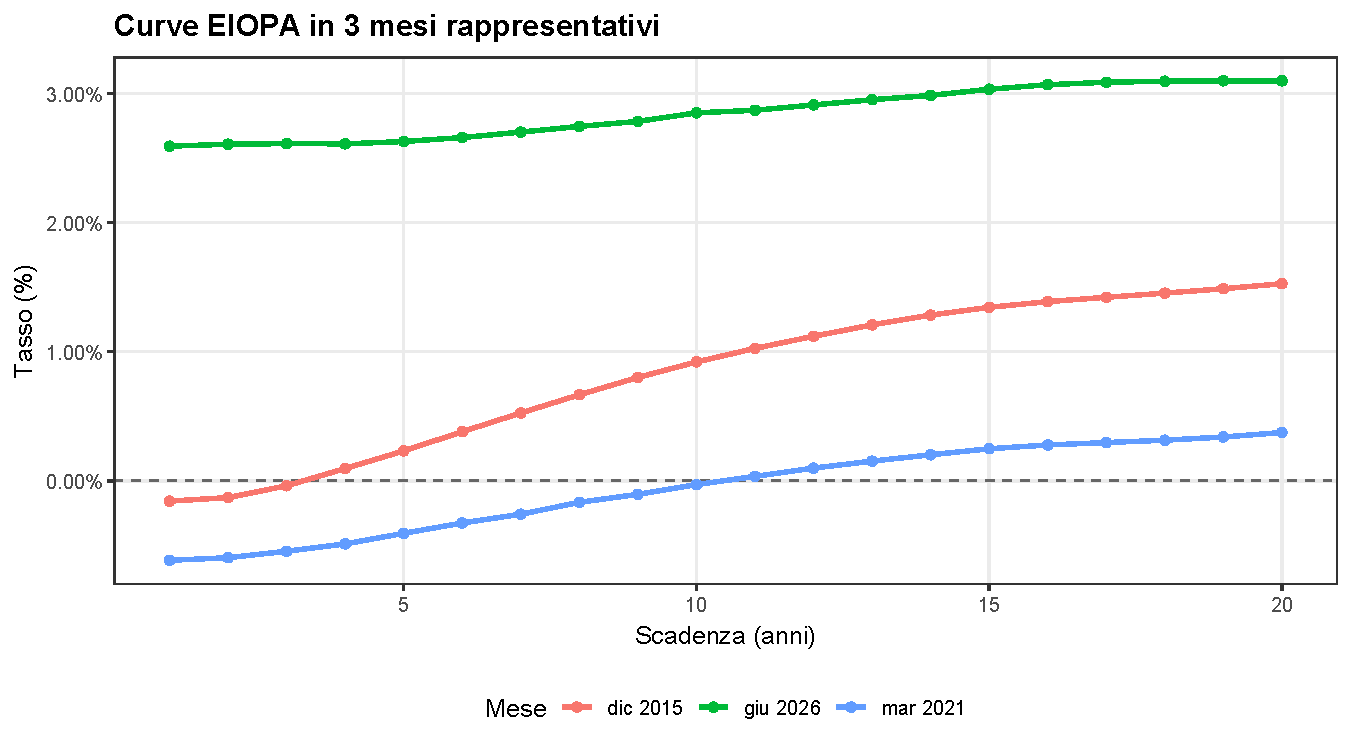
\includegraphics[width=0.92\textwidth]{../../output/03c_pca_eiopa/step1_curve_livelli_m.pdf}
\caption{Curve EIOPA in tre mesi rappresentativi del campione. L'asse $x$
indica la scadenza in anni, l'asse $y$ il tasso in \%. Si noti che nel mese
centrale la curva \`e \textbf{negativa} su buona parte delle scadenze: l'ultimo
mese del campione con tassi negativi nella finestra 1--20 anni \`e febbraio
2022. Questo \`e il motivo per cui l'analisi che segue \`e condotta su
variazioni \emph{assolute} (in punti base) e non relative: a livelli negativi o
prossimi a zero una variazione percentuale non \`e definita in modo utile.}
\end{figure}

\subsubsection{Variazioni mensili: la matrice \texorpdfstring{$\Delta R$}{Delta R}}

La PCA si applica alle \emph{variazioni} della curva, non ai livelli:
\[
(\Delta R)_{s,j} = R_{s,j} - R_{s-1,j},
\quad s = 2,\ldots,M,\; j = 1,\ldots,n.
\]

\medskip
Applicare la PCA ai livelli $R$ sarebbe tecnicamente possibile, ma
produrrebbe risultati statisticamente non affidabili per tre ragioni:

\begin{enumerate}
  \item \textbf{Non stazionarietà.}
        I tassi di interesse sono spesso modellati come moti browniani con drift e dunque applicare la PCA a una serie
        non stazionaria significa decomporre la varianza di un processo che
        non ha media e varianza costanti nel tempo: i loadings ottenuti
        dipenderebbero fortemente dal periodo campionario e non sarebbero
        generalizzabili. Le variazioni $\Delta R$ sono invece stazionarie
        (o quasi-stazionarie), e la PCA è uno strumento progettato per dati
        stazionari~\cite{litterman1991}.

  \item \textbf{Dominanza del livello medio.}
        Se si applica la PCA ai livelli, la prima componente cattura quasi
        interamente la traiettoria storica media dei tassi (la discesa verso i
        tassi negativi fino al 2021 e la risalita del 2022--2023): non un
        \emph{movimento} della curva, ma la sua \emph{tendenza secolare}.

  \item \textbf{Interpretazione in termini di rischio.}
        Nella gestione di portafoglio e nel calcolo del VaR, l'input naturale
        è la variazione di valore (P\&L), che dipende dalle variazioni dei tassi
        $\Delta r(T)$, non dai loro livelli. I tre fattori PCA estratti da
        $\Delta R$ --- livello, pendenza, curvatura --- hanno quindi un
        significato operativo diretto~\cite{rebonato2004}.
\end{enumerate}

\begin{warningbox}
\textbf{Nota pratica.} In letteratura si trovano a volte PCA sui livelli (es.\ per
costruire curve parametriche sintetiche). In quel contesto l'obiettivo è diverso:
si vuole approssimare la \emph{forma} della curva, non i suoi movimenti. Per
l'analisi del rischio e per la scomposizione fattoriale del P\&L, la PCA sulle
variazioni è lo standard consolidato fin da Litterman \& Scheinkman~\cite{litterman1991}.
\end{warningbox}

\begin{keybox}[Il CRA sparisce nelle variazioni]
Poich\'e il $\CRA$ \`e costante (10 pb) su tutti i 127 mesi del campione, esso
trasla rigidamente ogni curva di livello, ma \textbf{si elide esattamente} nella
differenza:
\[
  (R_s - \CRA) - (R_{s-1} - \CRA) = R_s - R_{s-1}.
\]
L'analisi che segue \`e dunque del tutto insensibile al $\CRA$. Non altrettanto
vale per l'$\UFR$, che nel campione cambia sei volte, n\'e per $\alpha$,
ricalibrato ogni mese: sono parametri \textbf{regolamentari} che variano nel
tempo e la cui variazione entra, sia pure in misura minima, nella matrice
$\Delta R$ che stiamo per decomporre.
\end{keybox}

\begin{figure}[H]
\centering
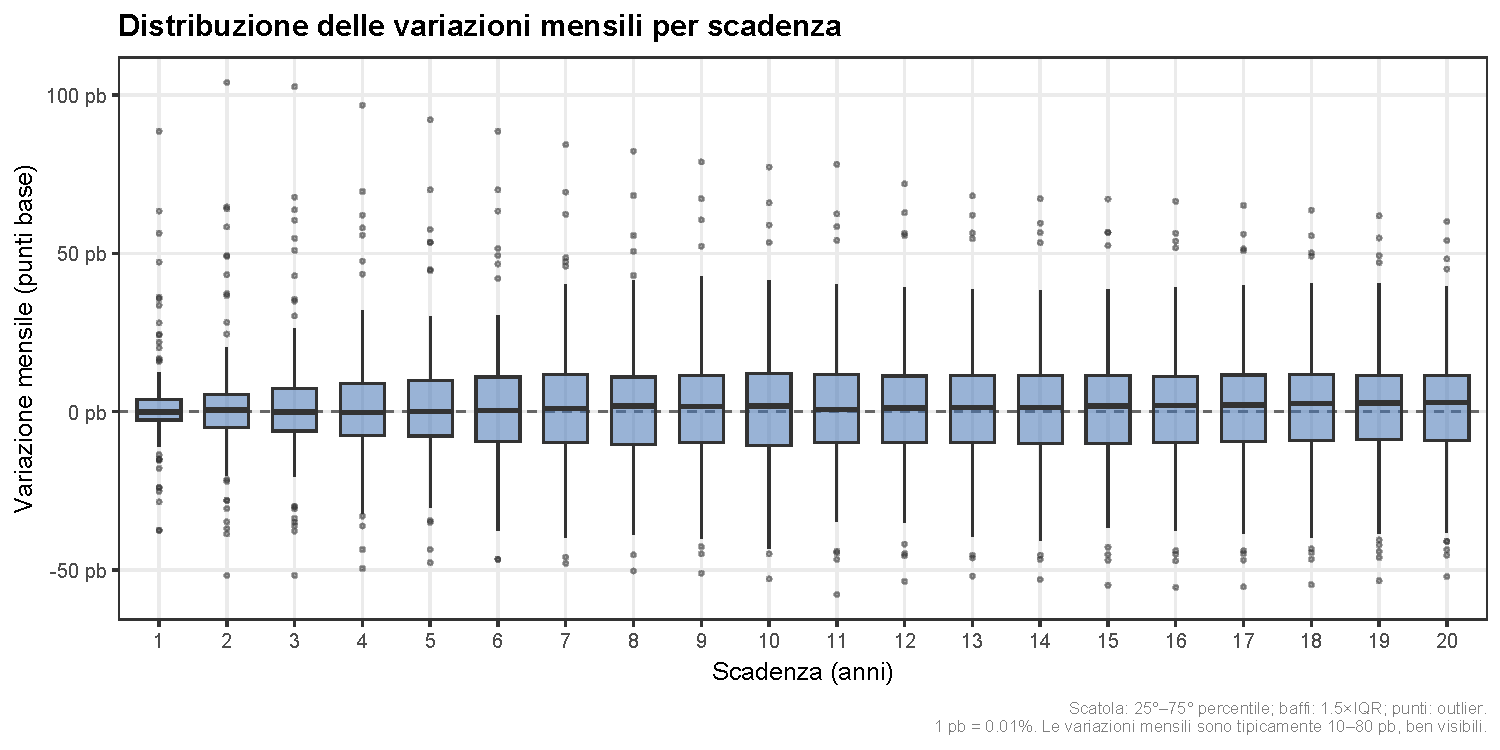
\includegraphics[width=0.95\textwidth]{../../output/03c_pca_eiopa/step1_delta_mensili_m.pdf}
\caption{\textbf{Distribuzione delle variazioni mensili} $\Delta R(T_j)$
per ciascuna scadenza, espressa in punti base (1~pb $= 0.01\%$). La
variabilit\`a \`e maggiore alle scadenze brevi e intermedie, dove si
concentrano i movimenti di pendenza e curvatura.}
\end{figure}

\subsubsection{Matrice di correlazione mensile}

\begin{figure}[H]
\centering
\begin{minipage}[t]{0.49\textwidth}
\centering
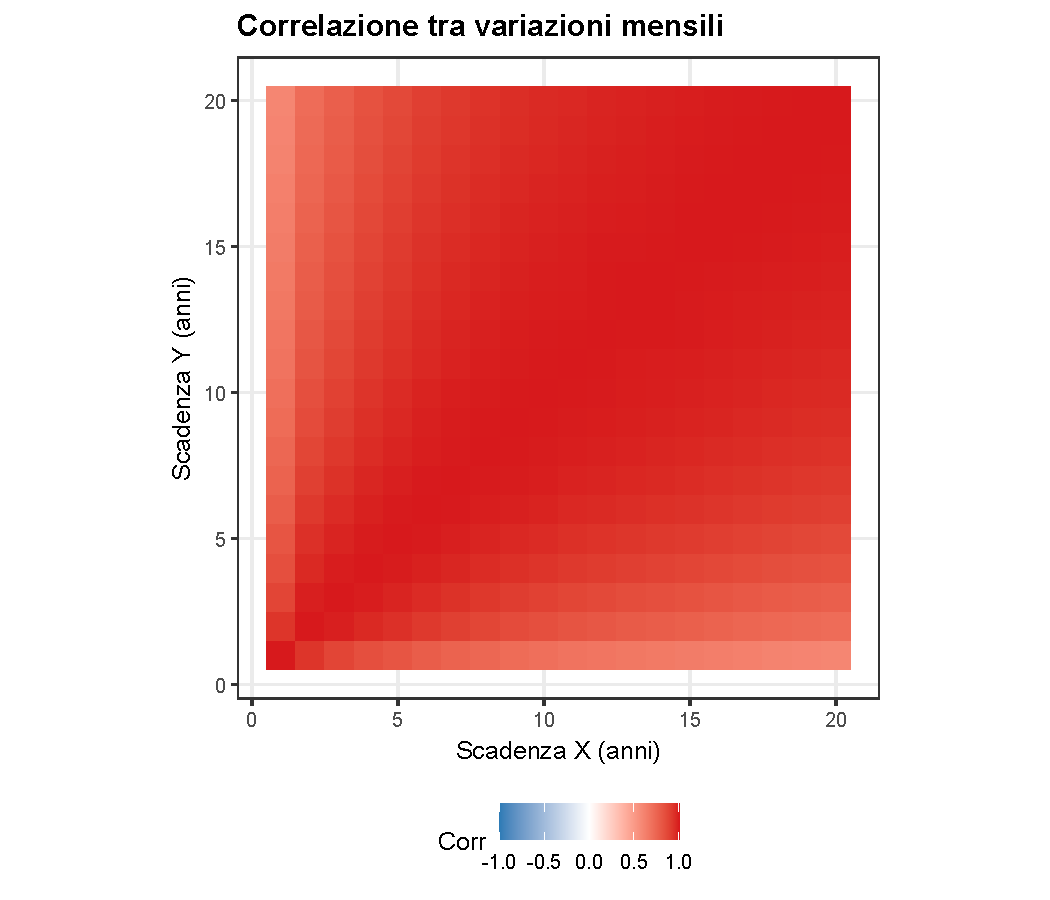
\includegraphics[width=\textwidth]{../../output/03c_pca_eiopa/step1_heatmap_correlazioni_m.pdf}
\end{minipage}\hfill
\begin{minipage}[t]{0.49\textwidth}
\centering
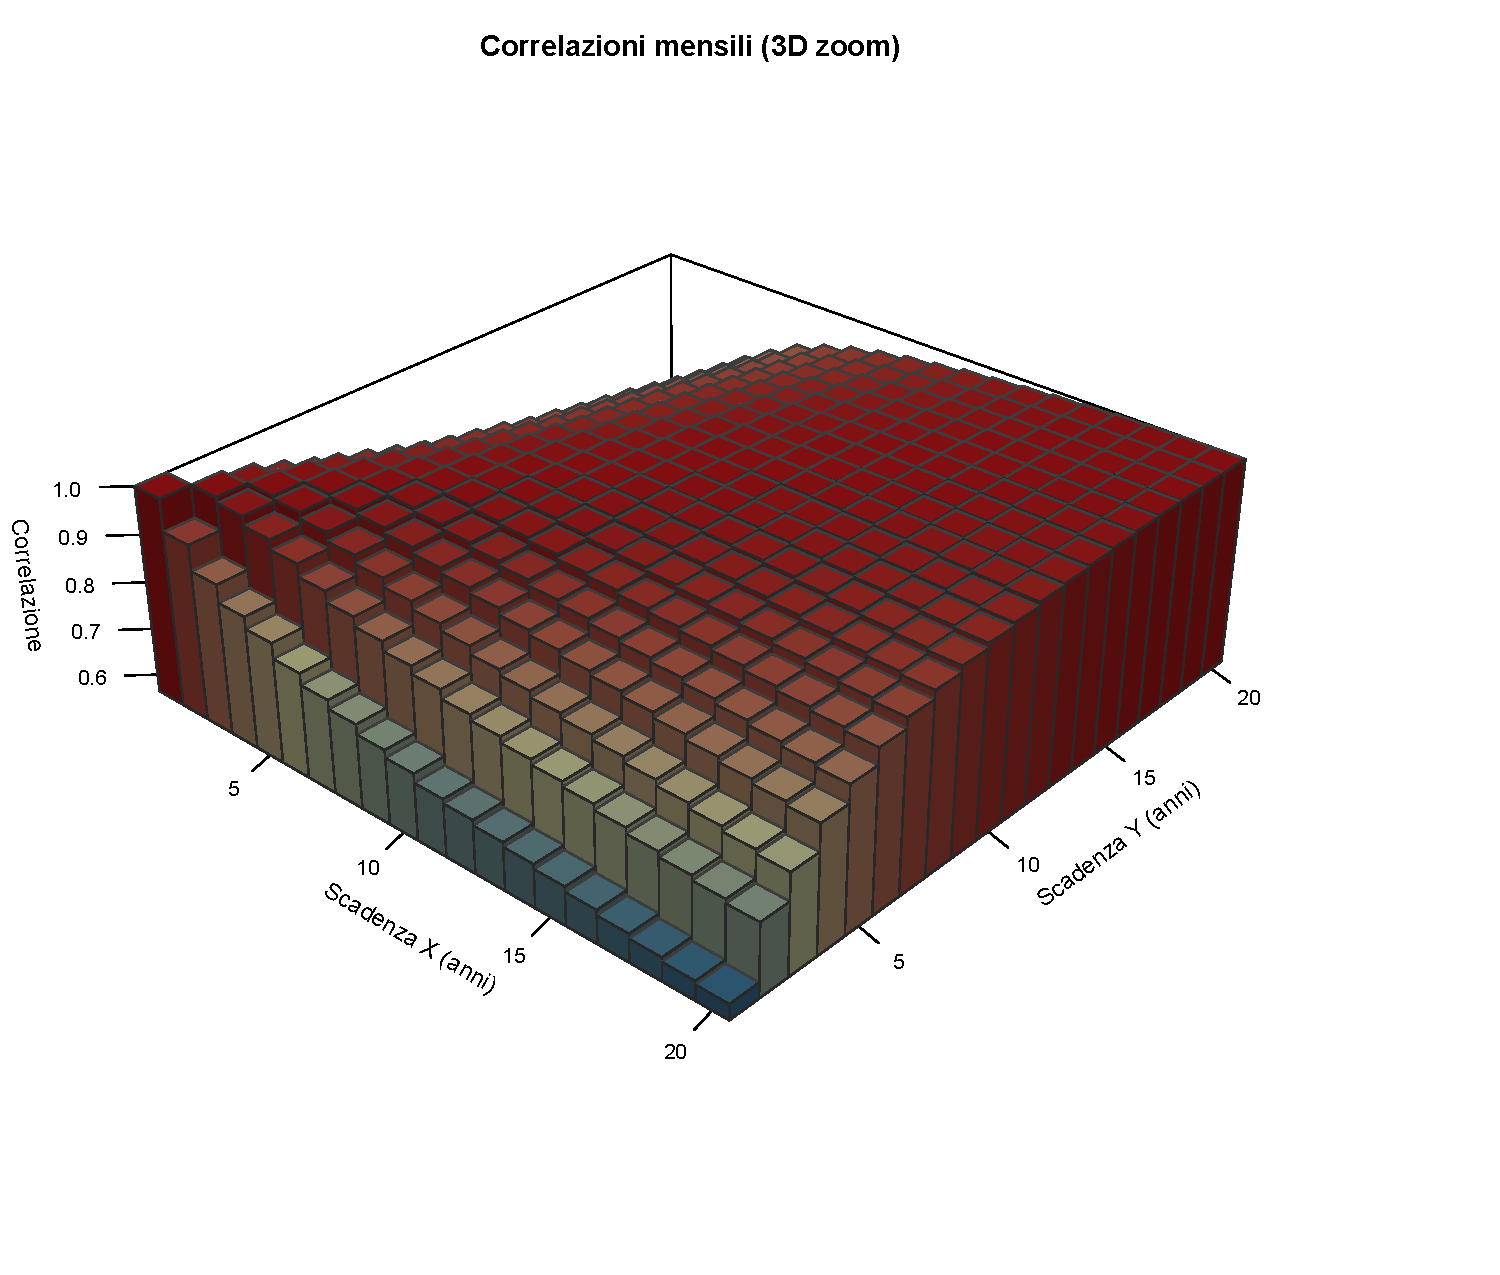
\includegraphics[width=\textwidth]{../../output/03c_pca_eiopa/step1_correlazioni_3d_barre_m.pdf}
\end{minipage}
\caption{Correlazione tra variazioni mensili visualizzata in due modi complementari:
heatmap (sinistra) e superficie a barre 3D (destra). Si osservi in particolare
la zona 12--20 anni: le scadenze 14, 16, 17, 18 e 19 non corrispondono a
strumenti quotati, ma sono prodotte dall'interpolazione Smith--Wilson a partire
dai nodi 13, 15 e 20.}
\end{figure}

% ------------------------------------------------------------
\subsection{PCA tramite SVD}
% ------------------------------------------------------------

\subsubsection{Costruzione della matrice centrata e SVD}

Applicando il Teorema~\ref{thm:pca} alla matrice mensile:

\begin{codebox}[Centraggio e SVD su dati mensili]
\begin{Verbatim}[fontsize=\small]
X_m      <- scale(Delta_R_m, center = TRUE, scale = FALSE)
sv_m     <- svd(X_m)

sing_vals <- sv_m$d
expl_var  <- sing_vals^2 / sum(sing_vals^2)
cum_var   <- cumsum(expl_var)
k_star    <- which(cum_var >= 0.95)[1]  # componenti per 95%
\end{Verbatim}
\end{codebox}

\begin{figure}[H]
\centering
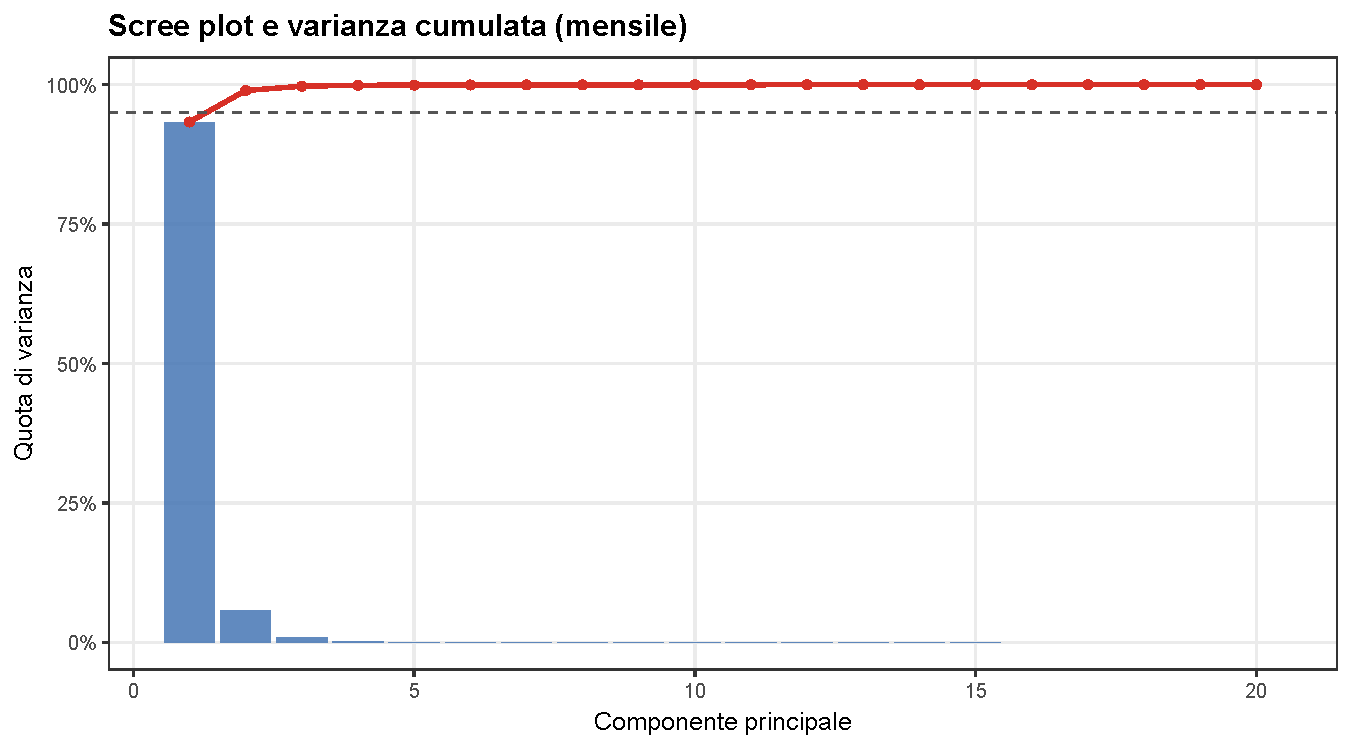
\includegraphics[width=0.92\textwidth]{../../output/03c_pca_eiopa/step2_varianza_spiegata_m.pdf}
\caption{Varianza per componente e varianza cumulata. Barre blu: varianza individuale per componente;
linea rossa: varianza cumulata; tratteggio grigio: soglia 95\%.}
\end{figure}

\begin{keybox}[Risultati numerici (generati da \texttt{R/03c\_pca\_eiopa.R})]
Campione mensile analizzato: \textbf{127} mesi e \textbf{20} maturity.
La soglia del 95\% di varianza spiegata \`e raggiunta con \textbf{2} componenti principali.
Varianza spiegata PC1--PC3: \textbf{93.31\%, 5.64\%, 0.78\%}.
Varianza cumulata con $k=3$: \textbf{99.74\%}.
RMSE della ricostruzione con $k=3$: \textbf{0.01036} (variazioni mensili in \%).
Mesi usati per il confronto (primo/centrale/ultimo): \textbf{gennaio 2016, marzo 2021, giugno 2026}.
Norme L$_2$ delle variazioni selezionate: \textbf{142.7, 30.6, 26.9~pb}.
Mese di movimento massimo del campione: \textbf{agosto 2022} (norma \textbf{354.8~pb}).

\end{keybox}

\noindent Nel seguito, in linea con la prassi consolidata in letteratura
(si veda la Sezione~\ref{sec:interpretazione}), si adotta $k^{*} = 3$: le prime
tre componenti principali spiegano una quota di varianza tale da rendere
trascurabile il contributo delle componenti residue.

% ------------------------------------------------------------
\subsection{Interpretazione e ricostruzione}
\label{sec:interpretazione}
% ------------------------------------------------------------

\subsubsection{I loadings: forma dei fattori sulla curva}

I loadings $\mathbf{v}_1, \mathbf{v}_2, \mathbf{v}_3 \in \mathbb{R}^n$
rappresentano le direzioni principali rispetto cui decomporre la variazione
mensile dei tassi di interesse.

\begin{figure}[H]
\centering
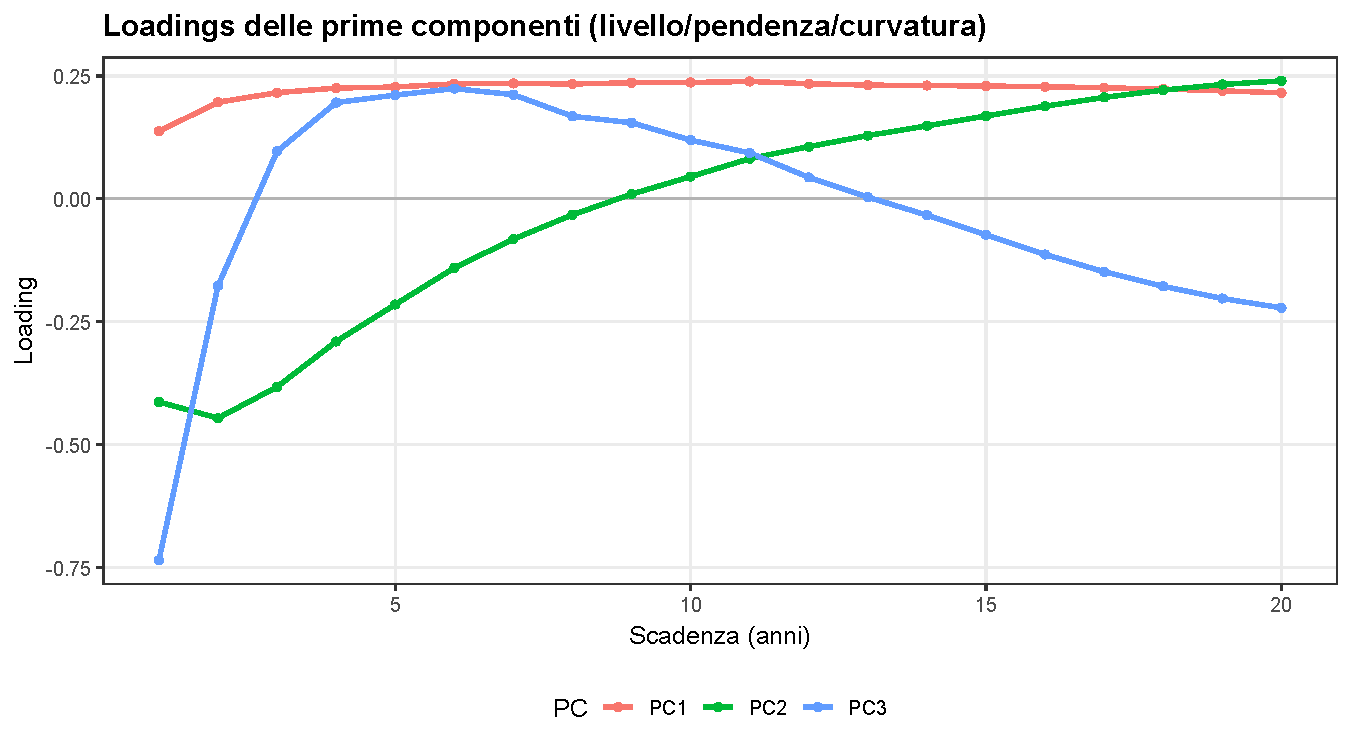
\includegraphics[width=0.92\textwidth]{../../output/03c_pca_eiopa/step3_loadings_pc1_pc3_m.pdf}
\caption{Loadings delle prime tre componenti in funzione della scadenza (anni).
PC1 piatta (livello), PC2 monotona (pendenza), PC3 a gobba (curvatura).}
\end{figure}

\subsubsection{Interpretazione economica dei tre fattori}

\begin{center}
\renewcommand{\arraystretch}{1.5}
\begin{tabular}{>{\bfseries}p{2.2cm} p{2.0cm} p{4.3cm} p{4.5cm} r}
\toprule
Fattore & Tipo & Forma del loading & Interpretazione & Var.\ tipica \\
\midrule
PC1 & Livello & Stesso segno e valore simile per tutte le scadenze &
Shift parallelo: tutti i tassi salgono o scendono insieme &
$70$--$90\%$ \\[4pt]

PC2 & Pendenza & Un cambio di segno: negativo (breve) / positivo (lungo) &
Rotazione: tassi brevi e lunghi in direzioni opposte &
$5$--$15\%$ \\[4pt]

PC3 & Curvatura & Due cambi di segno: positivo agli estremi, negativo al centro &
Butterfly: il ventre si muove in senso opposto agli estremi &
$1$--$7\%$ \\
\bottomrule
\end{tabular}
\end{center}

\noindent Gli intervalli riportati nell'ultima colonna sono quelli classici della
letteratura su curve di mercato~\cite{litterman1991}; i valori effettivi
calcolati sul campione EIOPA sono quelli riportati nel riquadro dei risultati
numerici.

\subsubsection{Gli scores mensili: la storia della politica monetaria BCE}

Dopo la decomposizione $\tilde X = U\Sigma V^T$, la matrice degli \textbf{scores}
è $A = U\Sigma \in \mathbb{R}^{(M-1)\times n}$, con $A_{s,i} = \sigma_i\, u_{s,i}$.
Lo score $\alpha_{s,i}$ misura \emph{di quanto} la curva si è mossa nel mese $s$
nella direzione del loading $\mathbf{v}_i$: un valore grande (in modulo) indica
che quel fattore ha dominato il movimento; un valore vicino a zero indica che
il fattore era inattivo.

\begin{figure}[H]
\centering
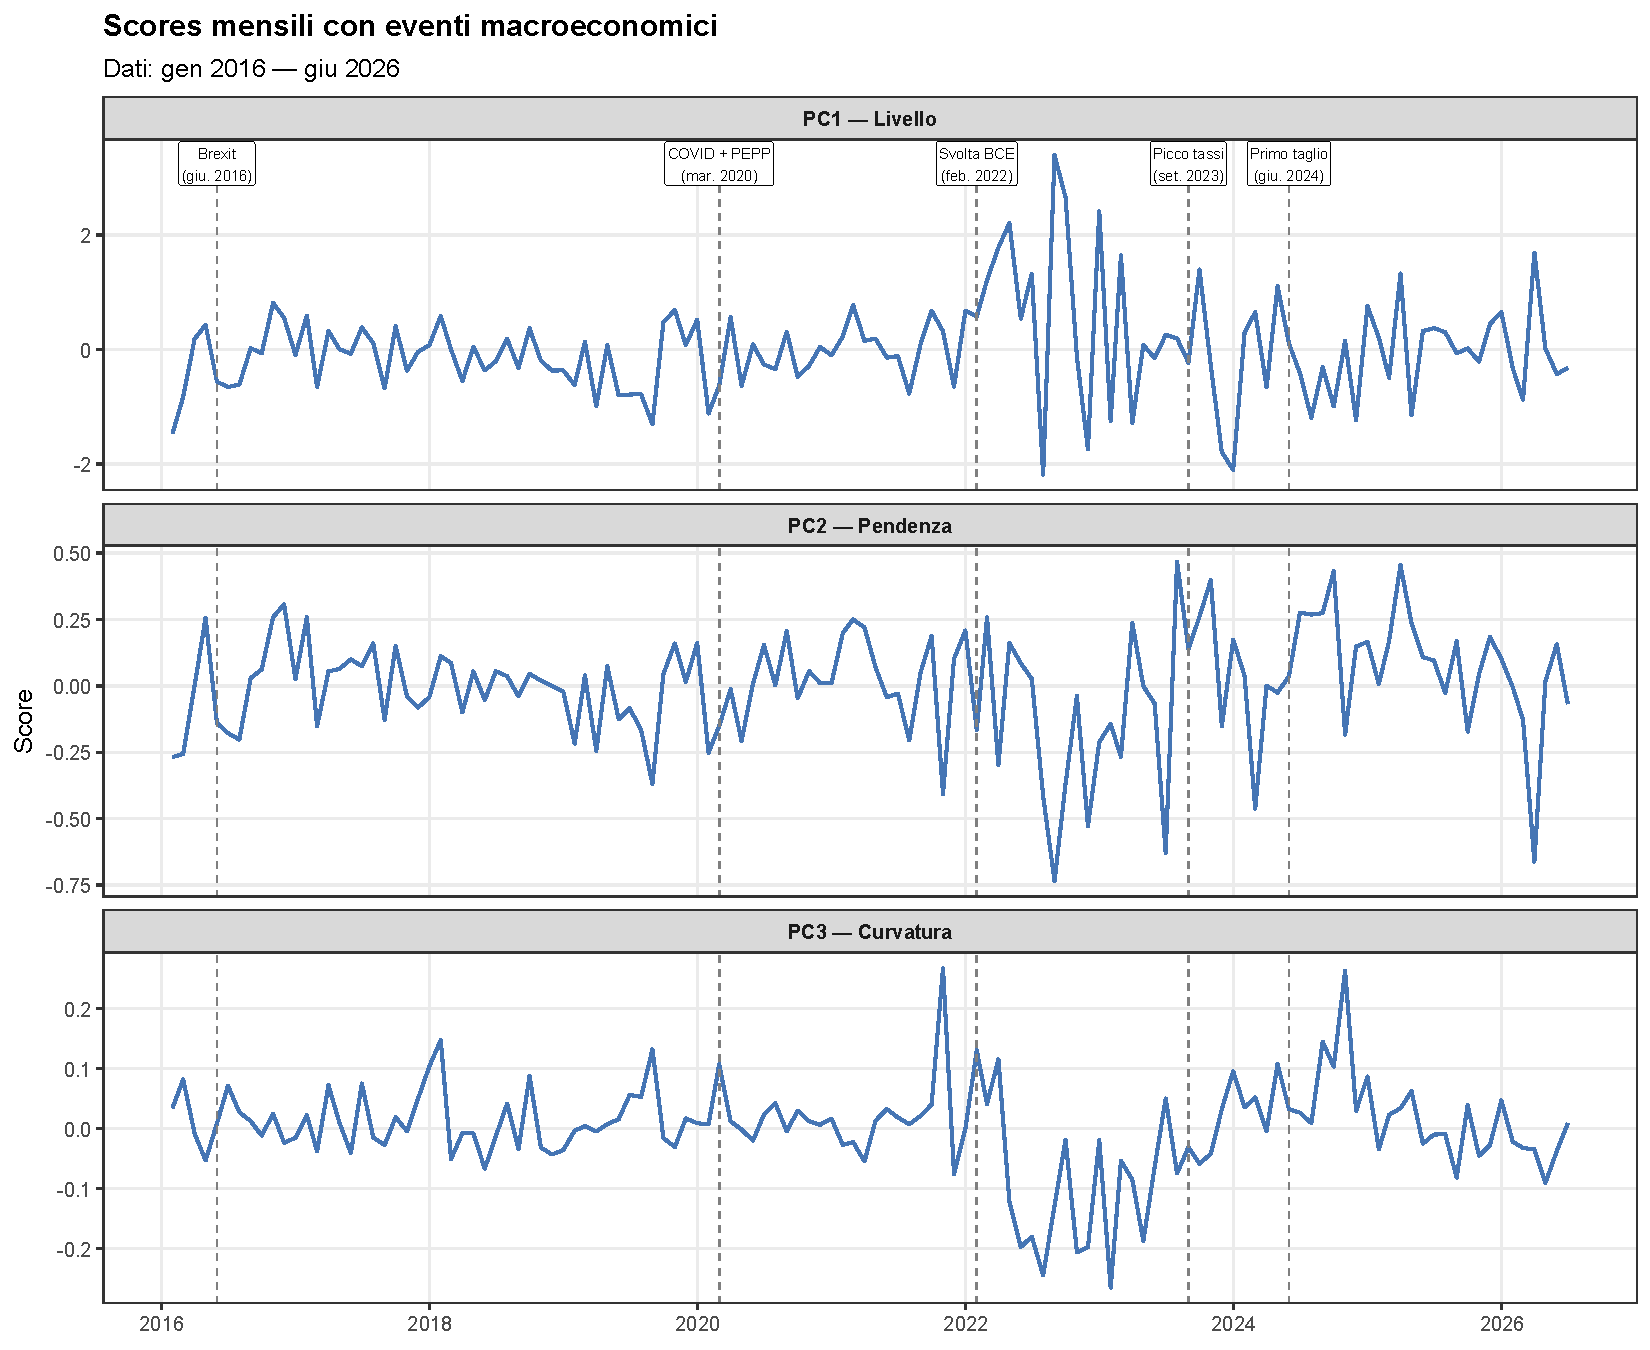
\includegraphics[width=0.97\textwidth]{../../output/03c_pca_eiopa/step3_scores_mensili_m.pdf}
\caption{Scores mensili PC1, PC2, PC3 con marcatura degli eventi macroeconomici
principali (linee tratteggiate grigie).}
\label{fig:scores_mensili}
\end{figure}

\noindent La Figura~\ref{fig:scores_mensili} riporta l'evoluzione temporale dei tre scores.
\textbf{PC1 (livello):} domina il ciclo di rialzi BCE del 2022--2023, il pi\`u
aggressivo dalla creazione dell'euro, che porta la curva fuori dal territorio
dei tassi negativi; i picchi negativi corrispondono invece alle fasi di
\emph{flight to quality} (Brexit 2016, shock pandemico 2020).
\textbf{PC2 (pendenza):} cattura i cambi di forma; nel 2022 la curva si
\emph{invertiva} (breve sopra lungo) mentre i tassi salivano --- PC2 segnala la
rotazione indipendentemente dal livello.
\textbf{PC3 (curvatura):} movimenti pi\`u piccoli ma identificabili, concentrati
nelle fasi di transizione della politica monetaria.

\begin{osservazione}
Si osservi che il picco di PC1 \textbf{precede} la prima decisione di rialzo
(luglio 2022) di alcuni mesi. Non \`e un'anomalia: la curva dei tassi prezza
\emph{aspettative}, non decisioni gi\`a prese. Gli scores PCA anticipano
sistematicamente le date ufficiali di politica monetaria.
\end{osservazione}

\subsubsection{Ricostruzione della curva}
\label{sec:ricostruzione}

La variazione mensile del mese $s$ si ricostruisce come combinazione lineare
dei loadings, pesati dagli scores:
\begin{equation}
  \hat{\Delta r}^{(k)}_s
  = \underbrace{\bar\delta}_{\text{media}}
  + \underbrace{\alpha_{s,1}\,\mathbf{v}_1}_{\text{livello}}
  + \underbrace{\alpha_{s,2}\,\mathbf{v}_2}_{\text{pendenza}}
  + \cdots
  + \alpha_{s,k}\,\mathbf{v}_k
  \label{eq:ricostruzione}
\end{equation}
dove $\bar\delta \in \mathbb{R}^n$ è il vettore delle variazioni medie
(sottratto prima della decomposizione SVD e aggiunto per riportare nella scala originale),
$\alpha_{s,i} = (U\Sigma)_{s,i}$ è lo score, e $\mathbf{v}_i$ il loading.

Consideriamo come esempio tre mesi --- il primo, quello centrale e l'ultimo del
campione --- per verificare la qualità della ricostruzione su periodi diversi.

\begin{figure}[H]
\centering
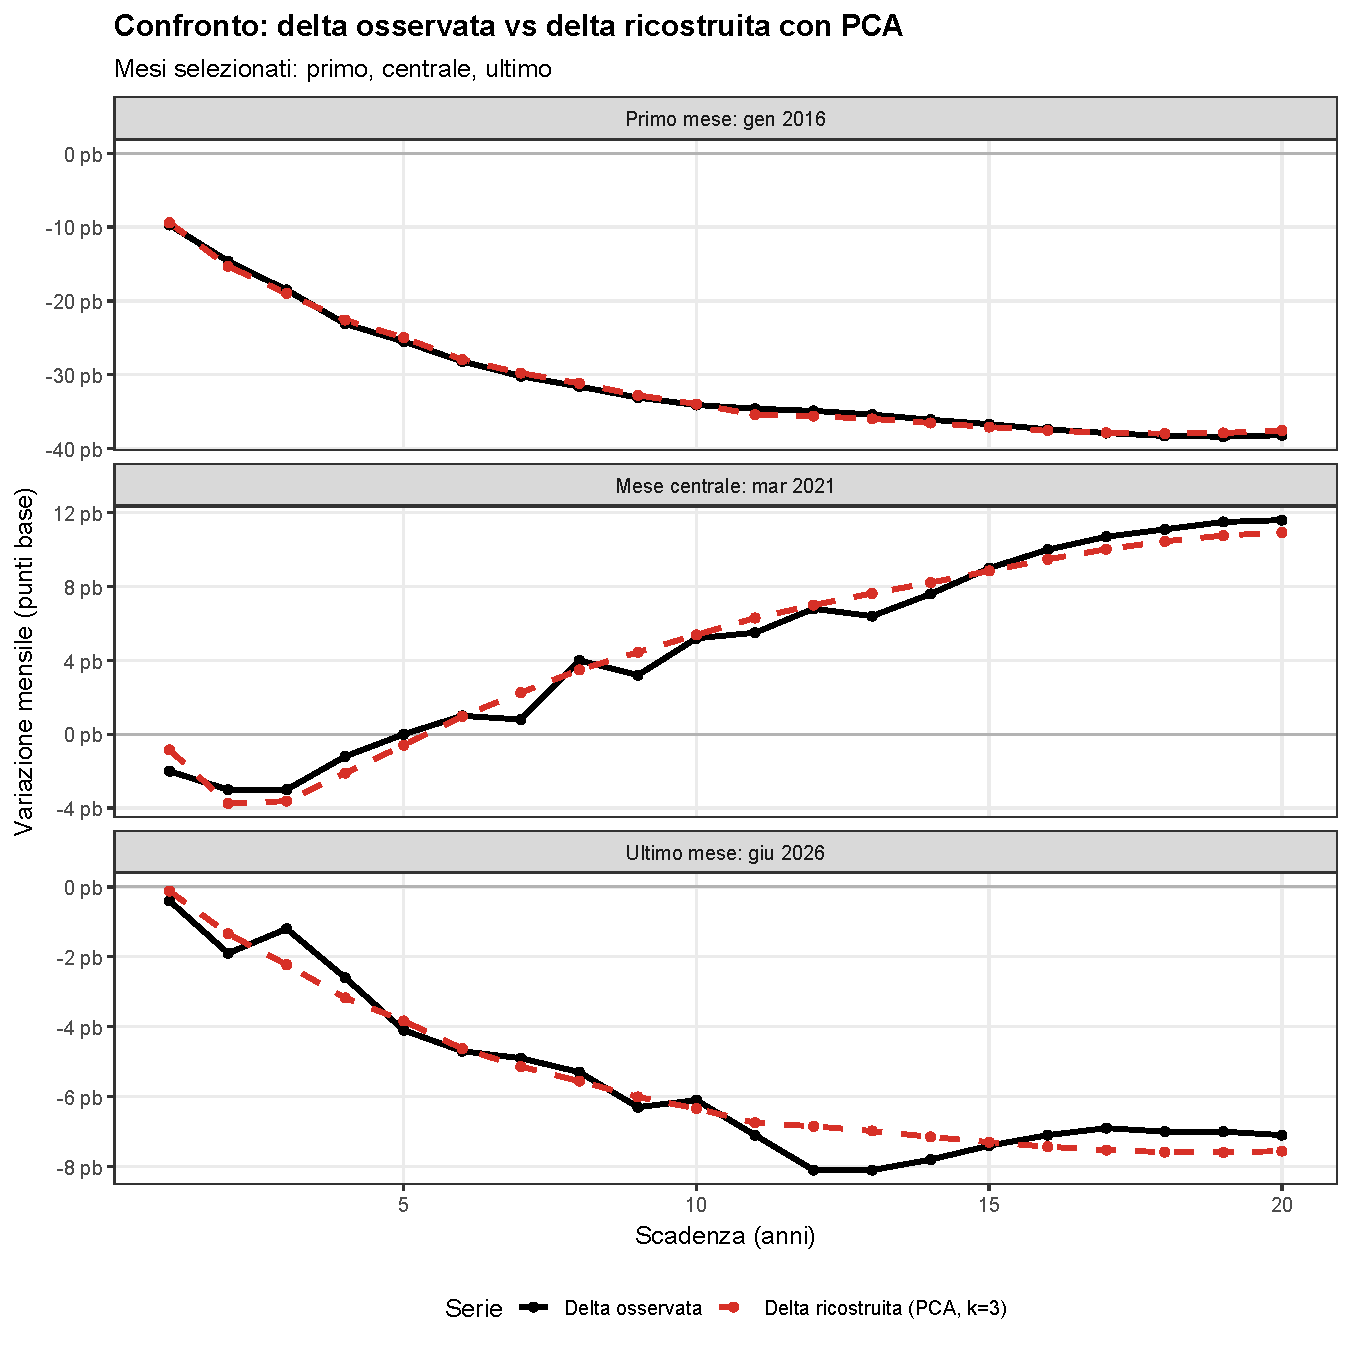
\includegraphics[width=0.8\textwidth]{../../output/03c_pca_eiopa/step3_confronto_ricostruzione_m.pdf}
\caption{Variazione mensile reale vs.\ ricostruita con $k=3$ componenti
nei tre mesi selezionati (primo, centrale, ultimo). L'asse $y$ è in punti base.}
\label{fig:confronto_ric}
\end{figure}

\noindent In ciascun pannello della Figura~\ref{fig:confronto_ric}, la curva osservata
e quella ricostruita sono molto vicine: la PCA a 3 fattori cattura i movimenti
principali della curva su tutta la storia del campione. Le discrepanze residue
sono associate alle componenti dalla quarta in poi, che spiegano una quota
limitata della varianza totale.

Per capire il contributo di ciascuna componente, è utile osservare come la curva
si ricostruisce aggiungendo un fattore alla volta. Come esempio concreto
utilizziamo il mese in cui la variazione della curva ha avuto la \textbf{norma
$L_2$ maggiore dell'intero campione}: il mese \`e selezionato automaticamente
dallo script ed \`e riportato nel riquadro dei risultati numerici.

\begin{figure}[H]
\centering
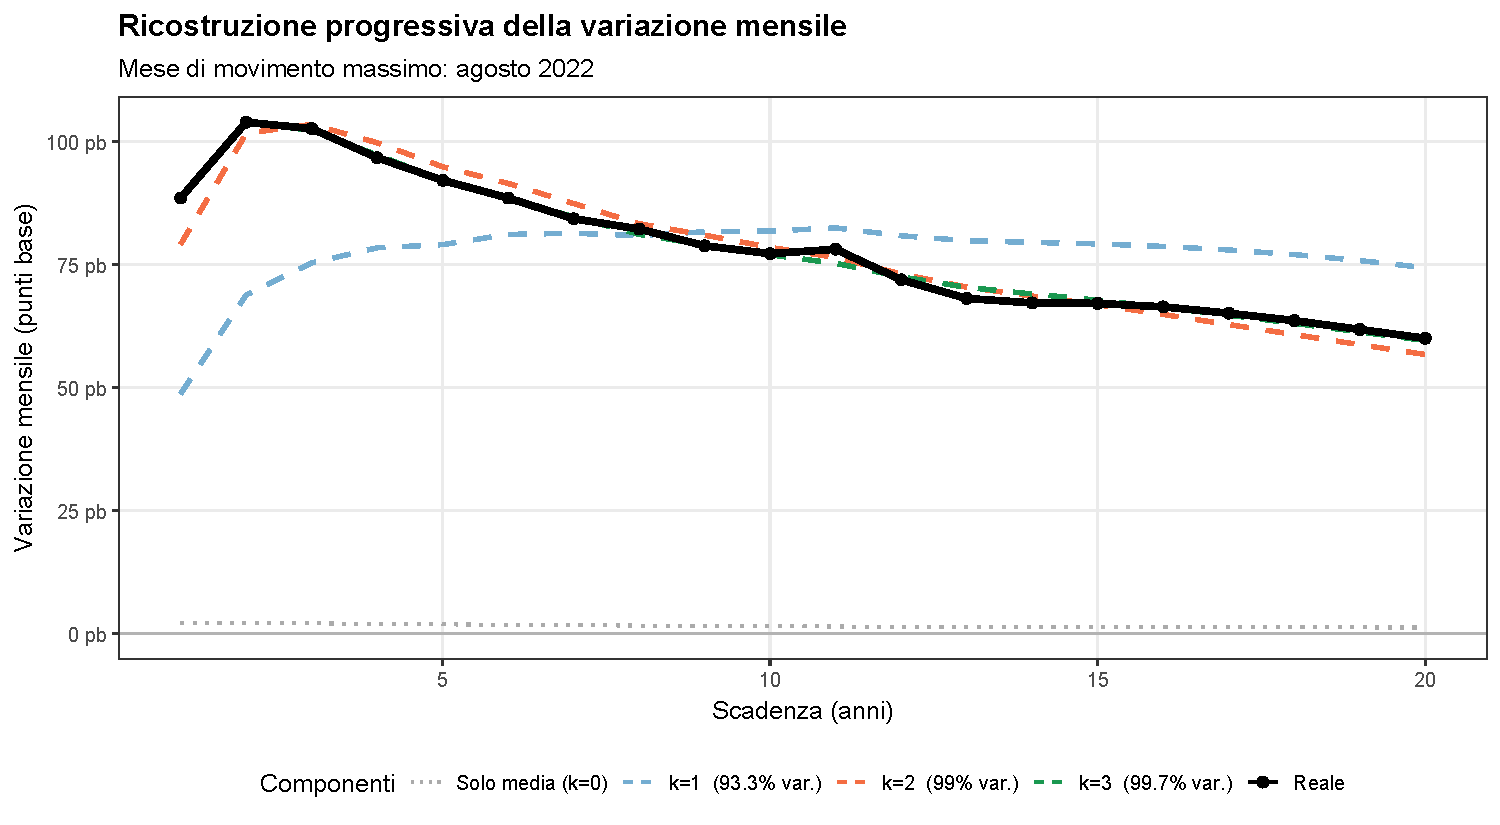
\includegraphics[width=0.97\textwidth]{../../output/03c_pca_eiopa/step3_ricostruzione_progressiva_m.pdf}
\caption{Ricostruzione progressiva della variazione mensile della curva EIOPA
nel mese di movimento massimo, aggiungendo una componente alla volta. La curva
nera è la variazione reale osservata (in punti base).}
\label{fig:ric_progressiva}
\end{figure}

\noindent La Figura~\ref{fig:ric_progressiva} mostra come ogni fattore contribuisce alla
ricostruzione.
\textbf{$k=1$ (+livello):} aggiunge lo shift parallelo dominante --- già la maggior
parte del movimento viene spiegata.
\textbf{$k=2$ (+pendenza):} corregge la rotazione breve-lungo, catturando la
differenza di movimento tra scadenze corte e lunghe.
\textbf{$k=3$ (+curvatura):} affina il profilo del ventre, riducendo ulteriormente
il residuo. La percentuale tra parentesi in legenda è la varianza cumulata spiegata
sull'intero campione da quella componente.

\subsubsection{Codice R: ricostruzione e selezione dei mesi rappresentativi}

\begin{codebox}[{Selezione automatica dei mesi: primo, centrale, ultimo}]
\begin{Verbatim}[fontsize=\small]
k_rec    <- 3L
scores_k_m   <- sv_m$u[, 1:k_rec] %*% diag(sv_m$d[1:k_rec], nrow=k_rec)
loadings_k_m <- sv_m$v[, 1:k_rec]
X_hat_m      <- scores_k_m %*% t(loadings_k_m)
rmse_m   <- sqrt(mean((X_m - X_hat_m)^2))

# Mesi selezionati: primo, centrale, ultimo
sel_month_idx <- c(1L, ceiling(nrow(Delta_R_m) / 2), nrow(Delta_R_m))
sel_month_ym  <- dates_delta_m[sel_month_idx]

# Mese di movimento massimo (ricostruzione progressiva)
row_norms <- sqrt(rowSums(Delta_R_m^2))
ref_idx   <- which.max(row_norms)

# Confronto reale vs ricostruita
mean_delta_m <- attr(X_m, "scaled:center")
delta_reale  <- Delta_R_m[sel_month_idx, ]
delta_rec    <- X_hat_m[sel_month_idx, ] +
                matrix(mean_delta_m, nrow =
                        length(sel_month_idx),
                        ncol = ncol(X_m),
                        byrow = TRUE)
\end{Verbatim}
\end{codebox}

% ------------------------------------------------------------
\subsection{Riepilogo dell'algoritmo completo}
% ------------------------------------------------------------

\begin{algobox}[PCA mensile della curva EIOPA (in R)]
\begin{Verbatim}[fontsize=\small]
# INPUT: 127 archivi zip in dati/eiopa_zips/

# 1. Estrazione: una curva per archivio (03c_pca_eiopa_prep.R)
#    zip -> EIOPA_RFR_<AAAAMMGG>_Term_Structures.xlsx
#        -> foglio RFR_spot_no_VA, colonna "Euro", scadenze 1..20
#    (nessuna aggregazione: il dato e' gia' mensile)

# 2. Matrice dei livelli e variazioni mensili
R_mat_m   <- as.matrix(curve_df[, ..maturity_cols])     # M x n
Delta_R_m <- diff(R_mat_m)                               # (M-1) x n

# 3. Centraggio per colonna
X_m <- scale(Delta_R_m, center = TRUE, scale = FALSE)

# 4. SVD della matrice centrata
sv_m <- svd(X_m)      # sv_m$u, sv_m$d, sv_m$v

# 5. Varianza spiegata
expl_var <- sv_m$d^2 / sum(sv_m$d^2)
cum_var  <- cumsum(expl_var)
k_star   <- which(cum_var >= 0.95)[1]

# 6. Loadings e scores
V_m    <- sv_m$v
scores_m <- sv_m$u[, 1:3] %*% diag(sv_m$d[1:3], nrow = 3)

# 7. Ricostruzione
X_hat_m      <- sv_m$u[, 1:3] %*% diag(sv_m$d[1:3], nrow=3) %*% t(sv_m$v[, 1:3])
sel_month_idx <- c(1L, ceiling(nrow(Delta_R_m) / 2), nrow(Delta_R_m))
\end{Verbatim}
\end{algobox}

% ============================================================
\section{Calibrazione degli scores su una curva arbitraria}
\label{sec:calibrazione}
% ============================================================

Una volta stimata la matrice dei loadings $V$ dalla PCA storica, è possibile
\emph{proiettare} qualsiasi nuova curva dei tassi $\mathbf{y} \in \mathbb{R}^n$
sullo spazio generato dalle prime $k$ componenti principali, ottenendo
$k$ \textbf{pesi} (scores) e una \textbf{ricostruzione approssimata}.
Con $k = n$ (base completa) la ricostruzione è esatta.

% ------------------------------------------------------------
\subsection{Proiezione ortogonale e pesi algebrici}
% ------------------------------------------------------------

Siano $\mathbf{v}_1, \ldots, \mathbf{v}_n \in \mathbb{R}^n$ i vettori colonna
di $V$ --- le colonne ortonormali della SVD di $\tilde{X}$, cioè i
\textbf{loadings PCA}. Essi formano una base ortonormale di $\mathbb{R}^n$:
\[
  V^T V = I_n, \qquad V \in \mathbb{R}^{n \times n}.
\]

Dati i primi $k \leq n$ loadings $V_k = [\mathbf{v}_1 \mid \cdots \mid \mathbf{v}_k]
\in \mathbb{R}^{n \times k}$, la ricostruzione di $\mathbf{y}$ con $k$
componenti si ottiene in due passi:

\begin{keybox}[Proiezione su $k$ componenti principali]
\textbf{Passo 1 --- Calcolo dei pesi (scores):} si proietta $\mathbf{y}$
su ciascuna direzione principale:
\[
  \boldsymbol{\alpha}_k = V_k^T\,\mathbf{y}
  = \begin{pmatrix} \mathbf{v}_1^T \mathbf{y} \\ \vdots \\ \mathbf{v}_k^T \mathbf{y} \end{pmatrix}
  \;\in\; \mathbb{R}^k.
\]
Ogni componente $\alpha_i = \mathbf{v}_i^T \mathbf{y}$ è il prodotto scalare
tra $\mathbf{y}$ e il loading $\mathbf{v}_i$: misura ``quanto'' di $\mathbf{y}$
sta nella direzione $i$-esima.

\medskip
\textbf{Passo 2 --- Ricostruzione:} si combinano linearmente i loadings
con i pesi appena calcolati:
\[
  \hat{\mathbf{y}}^{(k)} = V_k\,\boldsymbol{\alpha}_k
  = \alpha_1\,\mathbf{v}_1 + \alpha_2\,\mathbf{v}_2 + \cdots + \alpha_k\,\mathbf{v}_k
  \;\in\; \mathbb{R}^n.
\]
\end{keybox}

\paragraph{Formula compatta.}
Sostituendo $\boldsymbol{\alpha}_k = V_k^T \mathbf{y}$ nella ricostruzione:
\[
  \hat{\mathbf{y}}^{(k)} = V_k (V_k^T \mathbf{y}) = (V_k V_k^T)\,\mathbf{y}.
\]
La matrice $P_k = V_k V_k^T \in \mathbb{R}^{n \times n}$ è il \textbf{proiettore
ortogonale} sullo spazio generato dalle prime $k$ colonne di $V$.

\begin{osservazione}
Per $k = n$ vale $V_n V_n^T = I_n$ (base completa), quindi
$\hat{\mathbf{y}}^{(n)} = \mathbf{y}$ e l'errore di ricostruzione è zero.
La curva viene recuperata \emph{esattamente} combinando tutti i loadings.
\end{osservazione}

% ------------------------------------------------------------
\subsection{Applicazione: ricostruzione della curva BCE del 31 dicembre 2025}
% ------------------------------------------------------------

Consideriamo la curva dei livelli BCE (titoli di Stato area euro con rating AAA)
al 31 dicembre 2025, cio\`e l'ultima disponibile nel campione della
dispensa~03:

\begin{center}
\small
\renewcommand{\arraystretch}{1.15}
\begin{tabular}{cr @{\hspace{2em}} cr}
\toprule
Scadenza & \multicolumn{1}{c}{Tasso (\%)} & Scadenza & \multicolumn{1}{c}{Tasso (\%)} \\
\midrule
 1Y & 2.024 & 11Y & 3.028 \\
 2Y & 2.108 & 12Y & 3.100 \\
 3Y & 2.212 & 13Y & 3.164 \\
 4Y & 2.325 & 14Y & 3.222 \\
 5Y & 2.441 & 15Y & 3.272 \\
 6Y & 2.554 & 16Y & 3.317 \\
 7Y & 2.663 & 17Y & 3.355 \\
 8Y & 2.765 & 18Y & 3.388 \\
 9Y & 2.861 & 19Y & 3.416 \\
10Y & 2.948 & 20Y & 3.439 \\
\bottomrule
\end{tabular}
\end{center}

\begin{osservazione}
Si noti che stiamo proiettando una curva \textbf{BCE} --- titoli di Stato AAA,
stimata con Svensson, in capitalizzazione continua --- su una base costruita
dalle variazioni di una curva \textbf{EIOPA} --- swap, Smith--Wilson,
capitalizzazione annua. La base $V$ non ha mai ``visto'' una curva BCE. La
qualit\`a della ricostruzione misura quindi quanto i due mondi condividano la
stessa geometria. La dispensa~03 svolge l'esercizio speculare (curva EIOPA su
loadings BCE).
\end{osservazione}

\noindent Calcoliamo i pesi $\boldsymbol{\alpha}_k = V_k^T\mathbf{y}$ per $k = 1, \ldots, 20$
e le relative ricostruzioni.

Il Grafico~A (Figura~\ref{fig:sez5_livelli}) confronta la curva originale
con due ricostruzioni: $k = 3$ (approssimazione con i tre fattori economici)
e $k = 20$ (base completa, ricostruzione esatta). Già con sole 3 componenti
la forma della curva è catturata; con $k = 20$ la curva ricostruita
coincide esattamente con l'originale.

Il Grafico~B (Figura~\ref{fig:sez5_errore}) mostra l'errore $\varepsilon_k$
in punti base su scala logaritmica, per $k = 1, \ldots, 19$. La scala log
evidenzia il tasso di convergenza: l'errore decresce rapidamente nelle prime
componenti e diventa trascurabile oltre $k = 10$. Per $k = 20$ l'errore è
numericamente zero (non mostrato perché non rappresentabile in scala log).

Il Grafico~B aggrega l'errore in un'unica norma $\varepsilon_k$; il
Grafico~C (Figura~\ref{fig:sez5_errore_tenor}) lo scompone
\emph{scadenza per scadenza}, confrontando $k=3$ e $k=10$.

\begin{figure}[htbp]
  \centering
  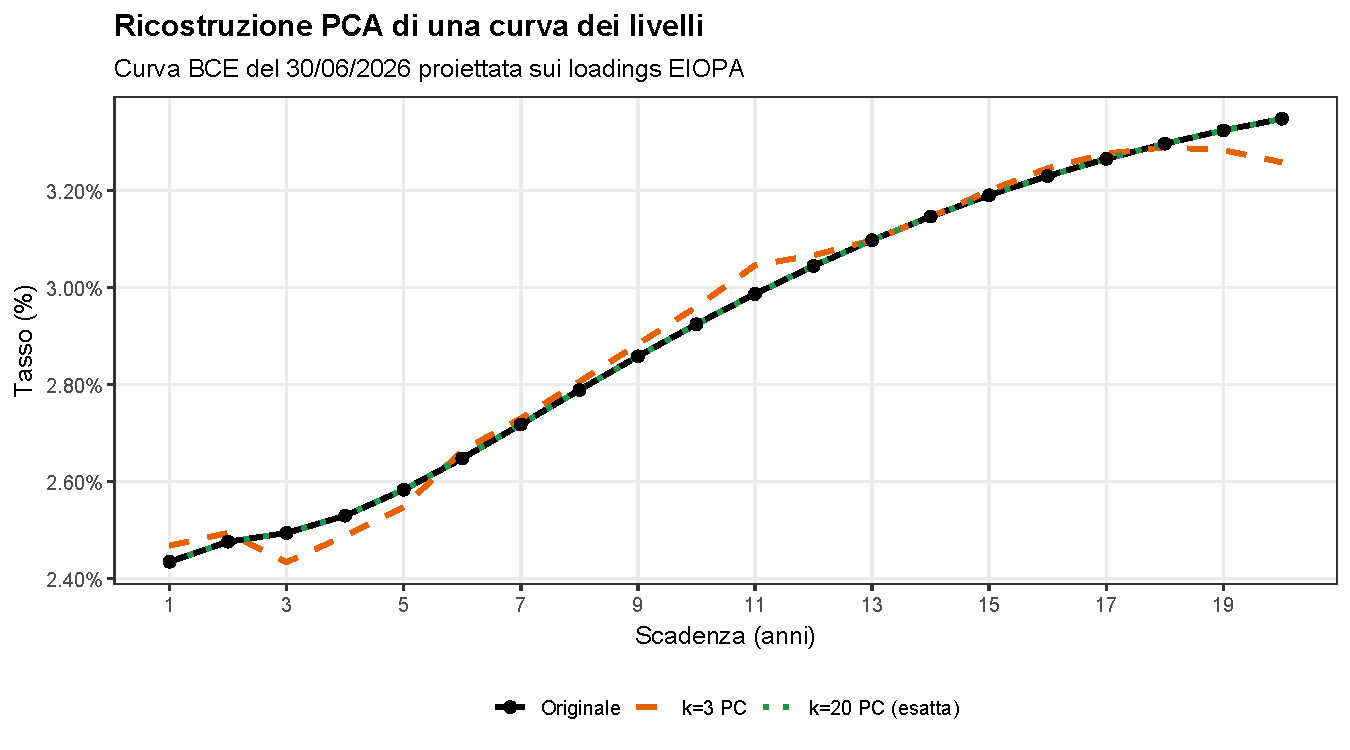
\includegraphics[width=0.88\textwidth]{../../output/03c_pca_eiopa/sez5_curva_ricostruzione.pdf}
  \caption{\textbf{Grafico A — Ricostruzione della curva dei livelli.}
    Curva nera con punti: originale (BCE, 31/12/2025). Curva arancio
    tratteggiata: ricostruzione con $k = 3$ componenti. Curva verde
    puntinata: ricostruzione con $k = 20$ (base completa).}
  \label{fig:sez5_livelli}
\end{figure}

\begin{figure}[htbp]
  \centering
  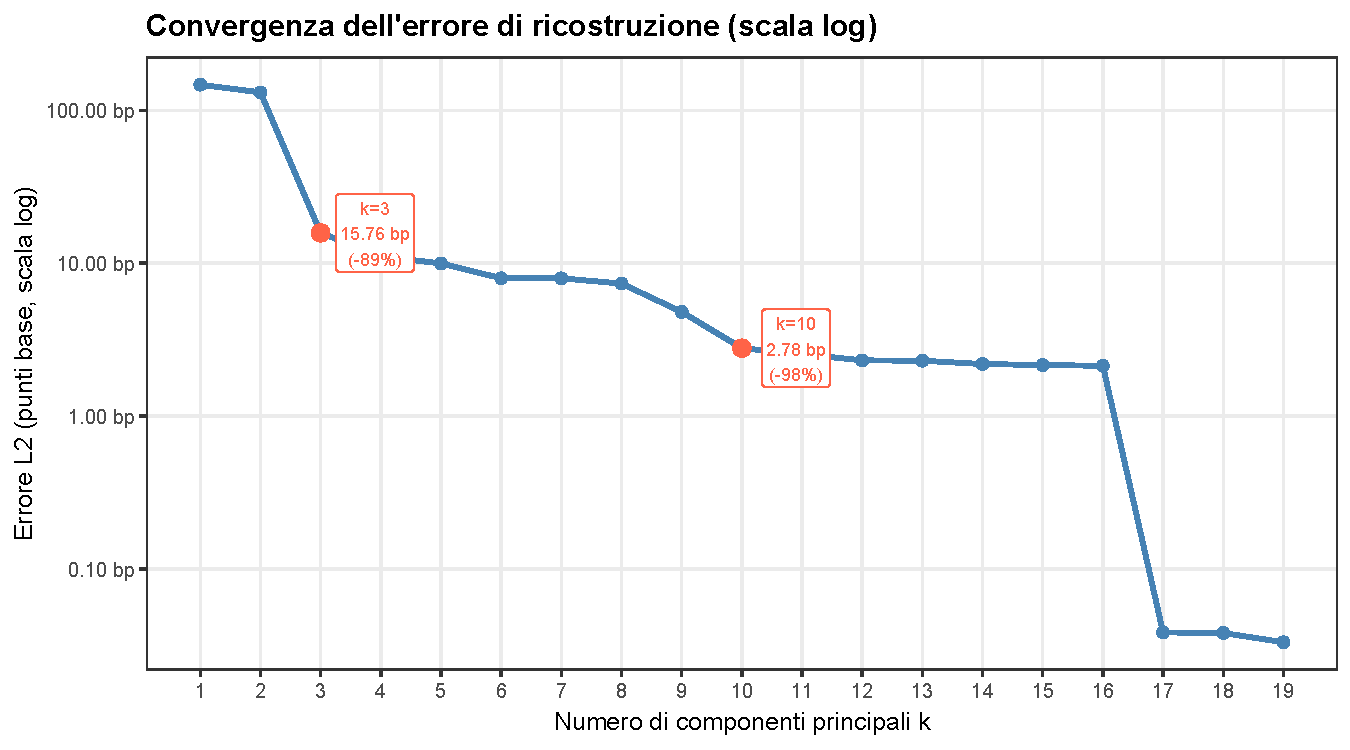
\includegraphics[width=0.88\textwidth]{../../output/03c_pca_eiopa/sez5_convergenza_errore.pdf}
  \caption{\textbf{Grafico B — Convergenza dell'errore (scala logaritmica).}
    Errore $\varepsilon_k = \|\hat{\mathbf{y}}^{(k)} - \mathbf{y}\|_2$ in punti
    base per $k = 1, \ldots, 19$. I punti rossi annotati indicano l'errore
    e la riduzione percentuale rispetto a $k = 1$ per $k = 3$ e $k = 10$.}
  \label{fig:sez5_errore}
\end{figure}

\begin{figure}[htbp]
  \centering
  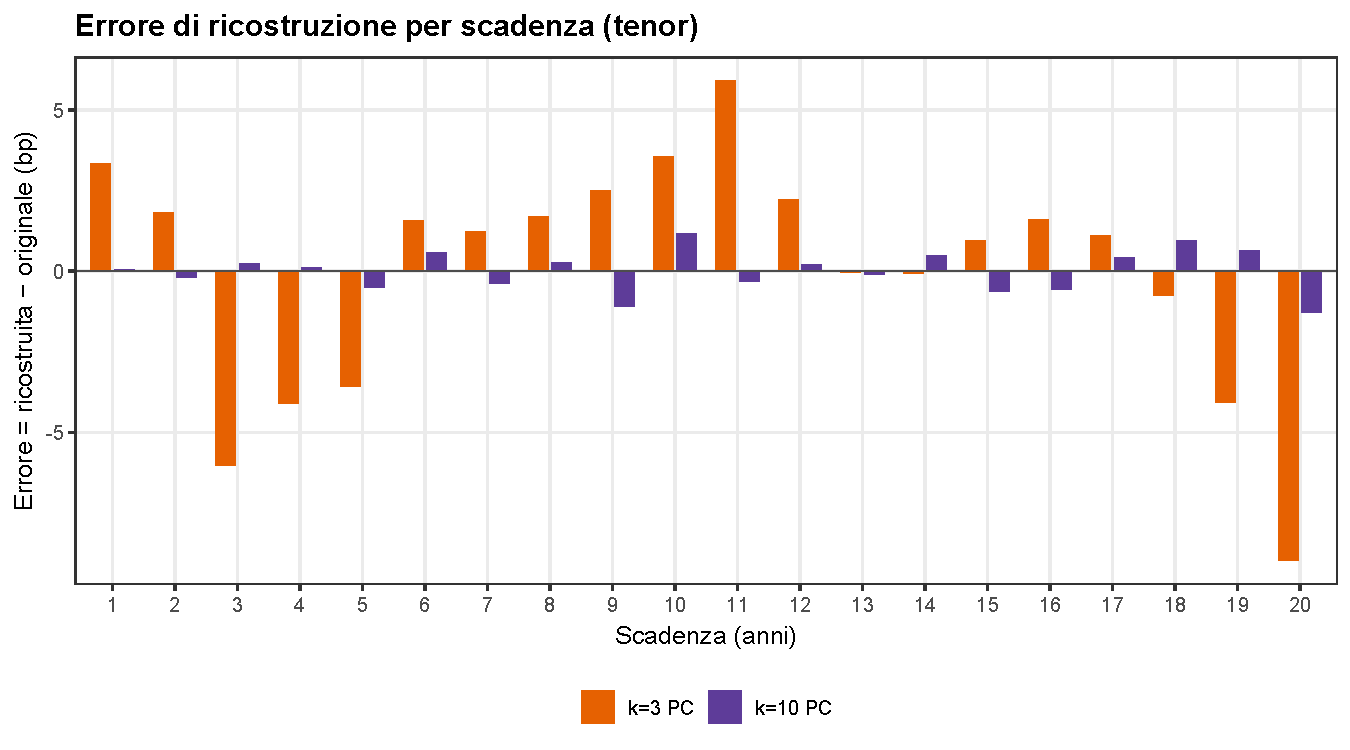
\includegraphics[width=0.88\textwidth]{../../output/03c_pca_eiopa/sez5_errore_per_tenor.pdf}
  \caption{\textbf{Grafico C — Errore di ricostruzione per singola scadenza.}
    Differenza (ricostruita $-$ originale) in punti base per ciascuna
    scadenza da 1 a 20 anni, con $k=3$ (arancio) e $k=10$ (viola)
    componenti principali.}
  \label{fig:sez5_errore_tenor}
\end{figure}

\newpage
% ------------------------------------------------------------
\section{Applicazioni pratiche}
% ------------------------------------------------------------

\begin{enumerate}
  \item \textbf{Compressione}: il dataset mensile (127 righe $\times$ 20 colonne)
        si riduce a 3 serie temporali di scores con perdita di informazione
        molto contenuta.
  \item \textbf{Scenari di stress}: uno shock di $+\sigma_1$ sul fattore
        livello identifica immediatamente la sensibilit\`a delle riserve
        tecniche a un movimento parallelo della curva di sconto. La PCA offre
        un'alternativa \emph{data-driven} allo shock di tasso della formula
        standard di Solvency~II, calibrata sulla storia effettiva della curva
        regolamentare.
  \item \textbf{Hedging fattoriale}: invece di coprirsi contro 20 movimenti
        indipendenti, si gestisce l'esposizione ai 3 fattori PCA mensili con
        soli 3 strumenti (es.\ swap EUR 2Y, 10Y, 20Y).
  \item \textbf{Previsione}: modelli VAR o ARIMA si applicano ai 3 scores mensili
        anzich\'e alle 20 variabili originali, con stime pi\`u stabili e
        interpretabili.
  \item \textbf{Generazione di scenari per l'ORSA}: si simulano i \textbf{3
        scores} (con un AR(1) oppure via bootstrap storico dei 126 vettori
        osservati) e si ricostruisce la curva completa a 20 scadenze tramite
        $\bar\delta + V_3\boldsymbol\alpha$. \`E l'approccio standard nei
        modelli interni: si simula in dimensione 3, si valuta in dimensione 20.
\end{enumerate}

% ============================================================
\section{Conclusioni}
% ============================================================

\begin{itemize}
  \item La PCA si applica alle \textbf{variazioni mensili centrate} $X$. Nel
        caso EIOPA la frequenza mensile non \`e una scelta dell'analista ma
        \`e imposta dal dato regolamentare, e coincide con quella rilevante
        per il bilancio delle imprese assicurative.
  \item Lo strumento matematico \`e la \textbf{SVD di $X$}: stabile, esatta,
        interpretabile tramite il Teorema di Eckart-Young.
  \item Le \textbf{prime 3 componenti} spiegano oltre il 99\% della varianza:
        il risultato \`e robusto e coerente con quanto osservato sulla curva
        BCE nella dispensa~03.
  \item I \textbf{loadings} rappresentano movimenti ben interpretabili della
        curva su tutte le maturity (livello, pendenza, curvatura); gli
        \textbf{scores mensili} sono leggibili e collegabili a eventi
        macroeconomici identificabili --- e, nel caso EIOPA, anche a
        \textbf{parametri regolamentari} oltre che a eventi di mercato.
  \item La finestra $1$--$20$ anni analizzata coincide con la parte
        \textbf{liquida} della curva: i risultati riguardano il mercato degli
        swap in euro e non l'estrapolazione verso l'$\UFR$, che \`e oggetto
        delle dispense~01 e~03.
\end{itemize}

% ============================================================
\renewcommand{\refname}{Riferimenti bibliografici}
\begin{thebibliography}{9}

\bibitem{quarteroni2017}
  \textbf{Quarteroni, A., Saleri, F., Gervasio, P.} (2017).
  \textit{Calcolo Scientifico}, 6a ed. Springer.
  Capitolo~6 per SVD e PCA.

\bibitem{burden2016}
  \textbf{Burden, R.L., Faires, J.D.} (2016).
  \textit{Numerical Analysis}, 10th ed. Cengage.

\bibitem{fabozzi2012}
  \textbf{Fabozzi, F.J.} (2012).
  \textit{Fixed Income Mathematics}, 4th ed. McGraw-Hill.
  Per il contesto obbligazionario dei fattori PCA.

\bibitem{litterman1991}
  \textbf{Litterman, R., Scheinkman, J.} (1991).
  \textit{Common Factors Affecting Bond Returns}.
  Journal of Fixed Income 1(1), 54--61.
  Articolo originale che identifica i 3 fattori (livello, pendenza, curvatura)
  nelle curve dei tassi USA.

\bibitem{rebonato2004}
  \textbf{Rebonato, R.} (2004).
  \textit{Volatility and Correlation: The Perfect Hedger and the Fox},
  2nd ed. Wiley Finance.
  Capitolo~7: analisi fattoriale delle curve dei tassi e applicazioni al
  risk management.

\bibitem{eiopa_rfr}
  \textbf{EIOPA} --- \emph{Risk-Free Interest Rate Term Structures}:
  \url{https://www.eiopa.europa.eu/tools-and-data/risk-free-interest-rate-term-structures}.
  Archivi mensili e documentazione tecnica.

\bibitem{eiopa_techdoc}
  \textbf{EIOPA} (2025). \textit{Technical Documentation of the Methodology to
  Derive EIOPA's Risk-Free Interest Rate Term Structures},
  EIOPA-BoS-25-599.

\bibitem{smithwilson2001}
  \textbf{Smith, A., Wilson, T.} (2001).
  \textit{Fitting Yield Curves with Long Term Constraints}.
  Bacon \& Woodrow Research Notes.

\bibitem{dispensa03}
  \textbf{Dispensa~03 del corso} --- \textit{EIOPA RFR: il metodo
  Smith--Wilson (approccio variazionale)}. Per la costruzione della curva,
  i nodi DLT, il $\CRA$ e l'estrapolazione verso l'$\UFR$.

\end{thebibliography}

\end{document}
